% Load document class

% possible options: color/nocolor, english/german, threecolumn
% default: color, english
\documentclass[english, leagacyboxes, nologo]{latex4ei/latex4ei_sheet}

\usepackage{upquote}

\begin{document}
\title{Network Security}
\author{Stephan Dollberg, Martin Zellner, Lucas Vandroux}
\myemail{lucas.vandroux@gmail.com}      % optional, delete if unchanged
\mywebsite{www.latex4ei.de}     % optional, delete if unchanged
\maketitle
\section{Introduction}

  \sectionbox{
  \subsection{Security Trends}
    Network security is an issue since \emph{critical infrastructures} in the open systems with a growing user base (\ra \emph{increasing risk}) are threatend by \emph{organized crime}.
  }
  \sectionbox{
  \subsection{Security Threats}
    \textbf{Asymmetric Threat:} Defenders must protect against all exploits on all systems but attackers can attack only a few.

    \textbf{Attacker Motivation:} Ego, Revenge, Destruction, Criminal intend, Aquisition of resources, Acquistion of sensitive information
  }
  \sectionbox{
  \subsection{Security Concepts}
    \textbf{CIA Triad}
    \begin{itemize}
      \item Confidentiality (prevention of unauthorized disclosure)
      \item Integrity (prevention of unauthorized modification or deletion)
      \item Availability (prevention of unauthorized withholding)
     \end{itemize}

     Also: Authenticity, Accountability(Responsability), Nonrepudiation (Can't deny), Privacy

     (Classification by Steve Kent)
     \textbf{Passive attacks:} Confidentiality (Content compromise, Traffic analysis)

     \textbf{Active attacks:} Availabilty (Denial of service), Integrity and Authenticity (Modification, Replay, Fabrication)

     \textbf{Secure Channel:} secure = authentic (of the sender) and confidential (no eavesdropping)

     \textbf{Security on OSI-Layers:} Physical (Link encryption), Network (IPSEC), Transport (SSL), Application (SSH)
   }
   \sectionbox{
   \subsection{OSI (Open Systems Interconnection)}
     \begin{tabular}{ | l | l | l |}
       \hline
       OSI Model & Data Seq. & Protocols + Port  \\
       \hline
       Application & Message & FTP 20-21, SSH 22, Telnet 23 \\
       \cline{1-1}
       Presentation* & & SMTP 25, HTTP/s 80/443 \\
       \cline{1-1}
       Session* & & DHCP, NTP, BGP 179 \\
       \hline
       Transport & Segment & TCP, UDP\\
       \hline
       Network & Datagram & IP, IPSec, ICMP, IGMP\\
       %& & ARP, ICMP \\
       \hline
       Data Link* & Frames & Ethernet, ARP\\
       \cline{1-2}
       Physical  & Bit Stream & 802.11 (WiFi)\\
       \hline
     \end{tabular}\\
     * \textit{Don't exist in TCP/IP Model}
   }

 \sectionbox{
 \subsection{ARP (Address Resolution Protocol)}
 % TODO is ARP link layer or Network layer protocol ?

 }

 \sectionbox {
 \subsection{HTTP (Hypertext Transfer Protocol)}
   \begin{itemize}
     \item Stateless protocol (Server doesn't know which client connects again)
     \item Status Code : 1xx info, 2xx success, 3xx redirection, 4xx client error, 5xx server error
     \item HTTP methods : GET, POST, PUT, DELETE, HEAD
     \item HTTP cookie : name$\leftrightarrow$value (expiration date, stored by client)
     \begin{itemize}
       \item Use for session management, secure cookie (HTTPS only)
     \end{itemize}
   \end{itemize}
 }


\section{(In)securtity, Risk and the Lifecycle of Vulnerablities}

  \sectionbox{
  \subsection{(In)security Landscape}
    General: complexity is bad (but increases fast)

    Security of a system := Security of its weakest link
  }
  \sectionbox{
  \subsection{Vulnerablity Lifecycle}
    \textbf{Security vulnerability} \\
    a weakness in a system allowing an attacker to violate the confidentiality, integrity, availability of the system or the data and applications it hosts

    disagreement on what is a vulnerability possible (it's a a feature not a vulnerability)

    \textbf{CVE}
    Standard names for all publicly known vulnerabilities and security exposures. De facto standard.

    Form: \emph{CVE-Year-AnyDigits}

    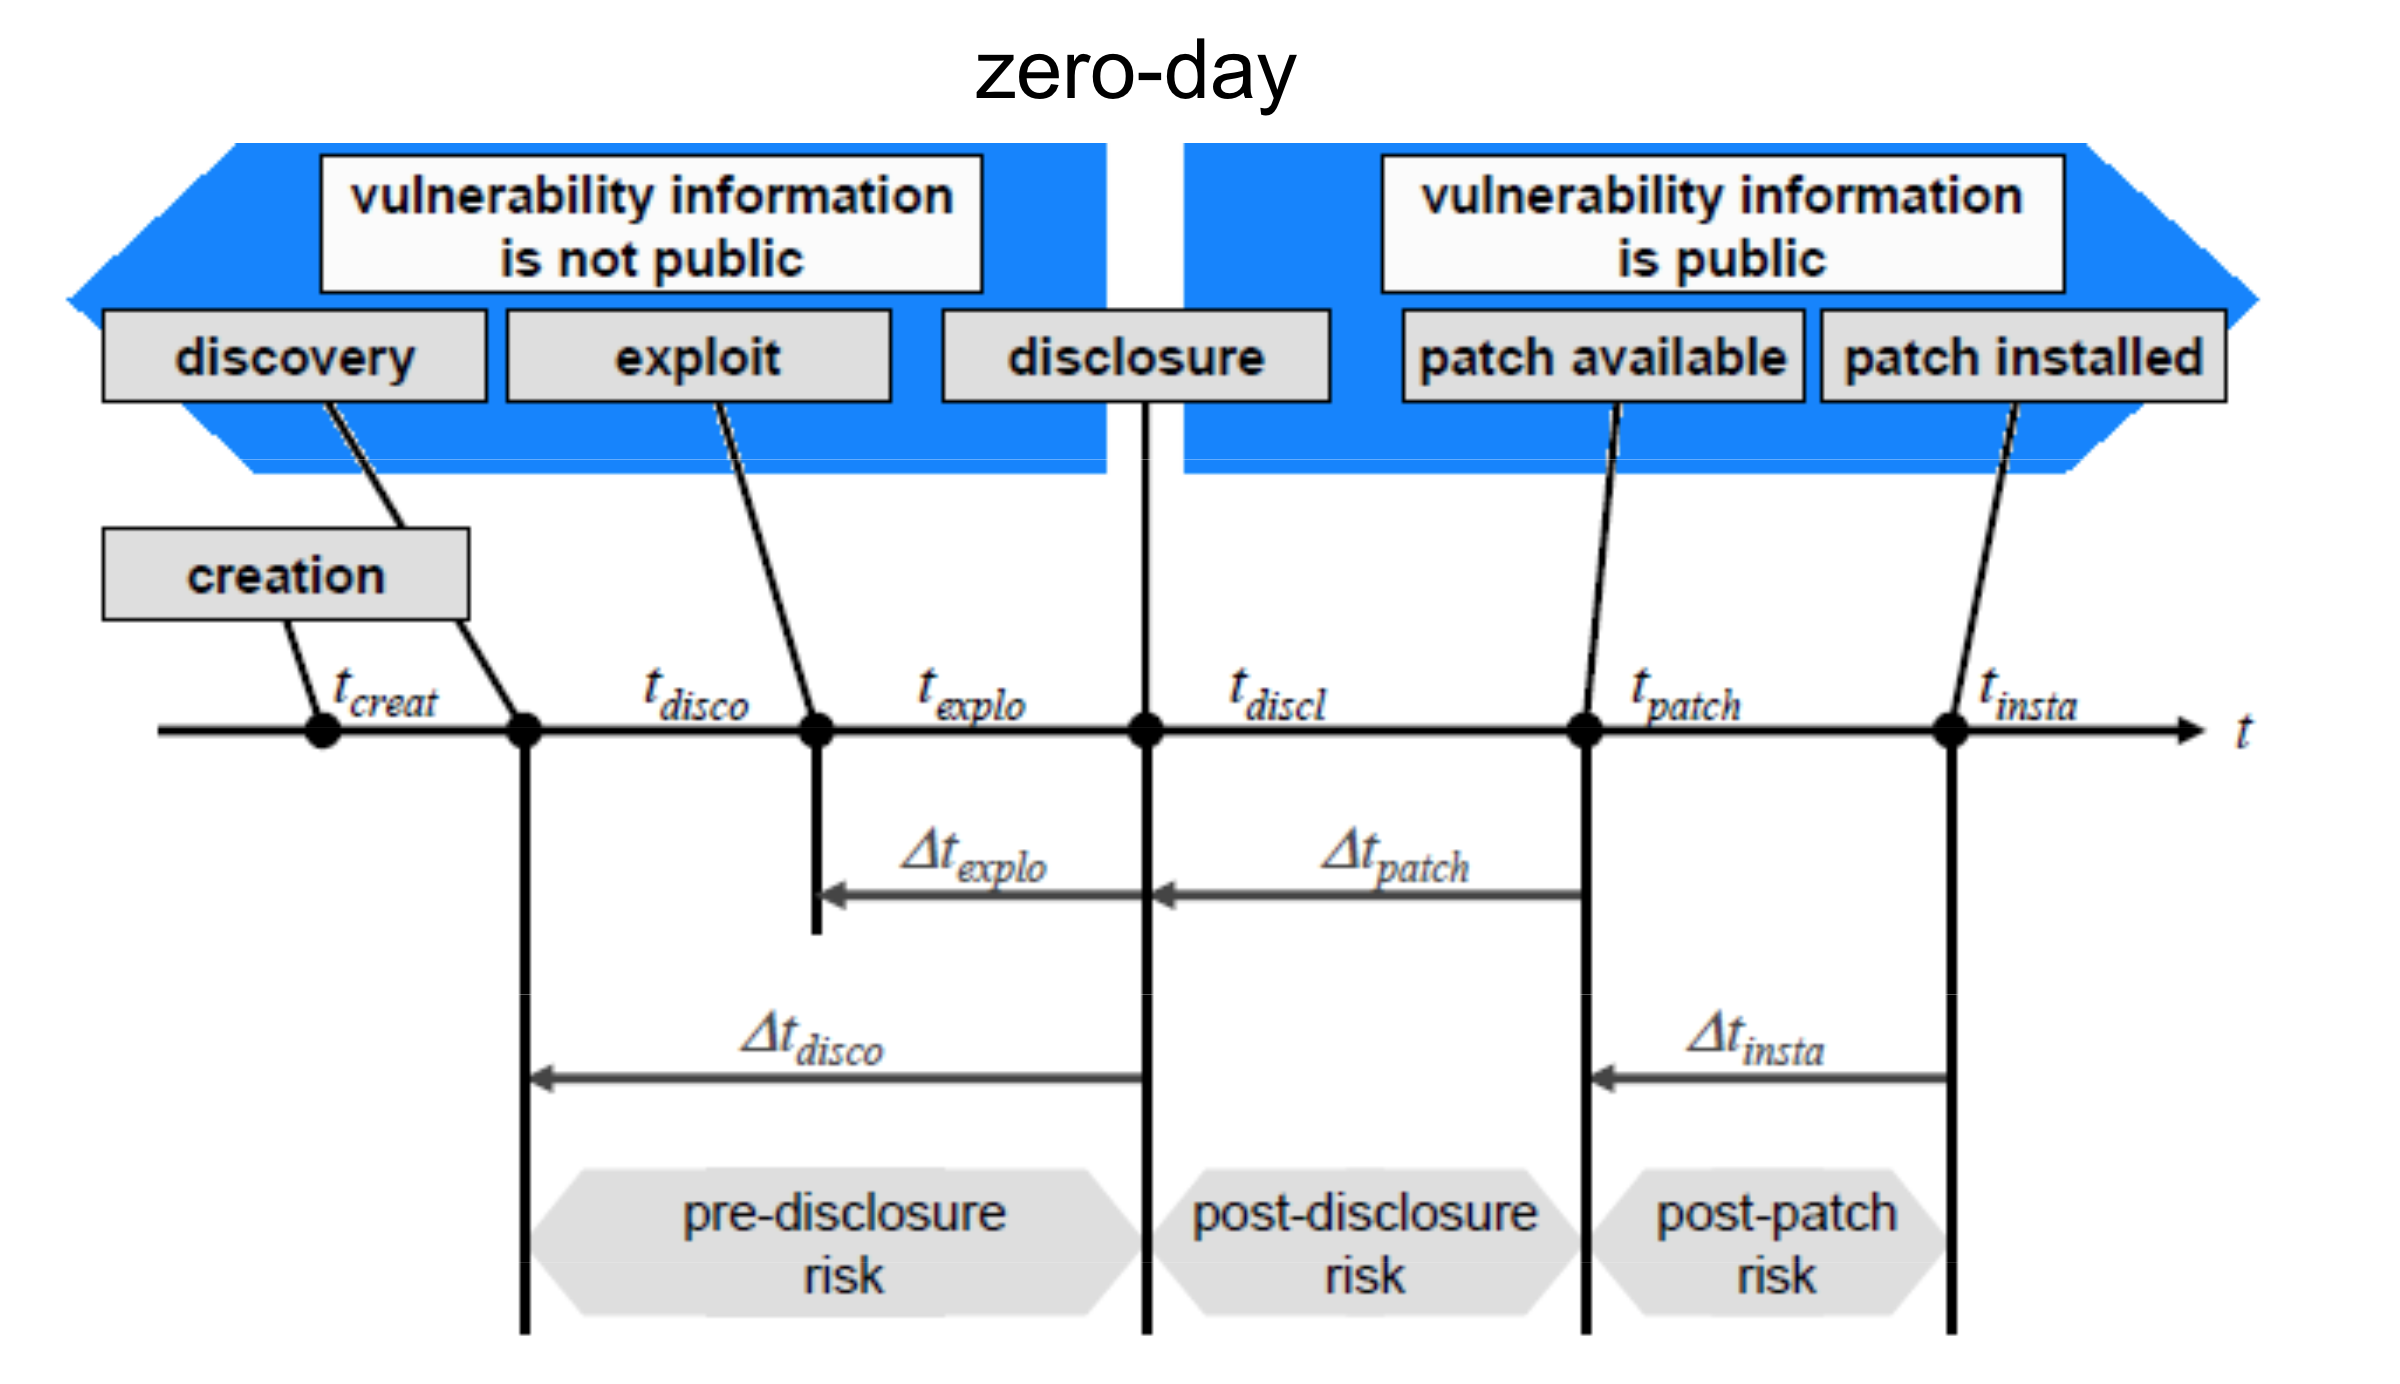
\includegraphics[width=\columnwidth]{img/VUL-LC.png}

    \textbf{Numbers:}\\
    50 \% of vulnerabilities known to insiders 30 or more days before disclosure (less-than-zero-day)

    At disclosure:  $\approx 50 \%$ unpatched

    A month after disclosure: $\approx 50 \%$ unpatched \\

    \textbf{Zero-day} Date when the vulnerability becomes known by the public

    \textbf{Zero-day-exploit} Attack that exploits a previously unknown vulnerability
  }
  \sectionbox{
  \subsection{Dynamics of (In) Security}
    \begin{itemize}
      \item extremely high dynamics around the disclosure
      \item exploit availability stays higher than the patch availability
      \item insiders: may know undisclosed vulnerabilites
    \end{itemize}

    \textbf{Gap of insecurity:} Difference between the exploit and patch (the bad a consistently faster than the good)
  }

  \sectionbox{
  \subsection{Risk}
    There is no such thing as absolute security

    Trade-Off between security and financial, social, functional, \ldots

    \subsubsection{Risk analysis}
    \begin{itemize}
      \item What assets are we trying to protect?
      \item what are the risk to those assets?
      \item How well does the security solution mitigate those risks?
      \item What other risks does the security solution cause?
      \item What costs and trade-offs does the security solution impose?
    \end{itemize}
    \ra is the trade-off worth if?

    \subsubsection{Risk management}
    Security is relative \Ra manage risks

    Options: avoid, decrease, transfer, accept risk

    Business sense: risk $<$ opportunity
  }


\section{Identity and Authentication}
  \sectionbox{
  \subsection{Identity and Identity Theft}
    \textbf{Authentication:} Authentication is the process of verifying an identity claim of an entity. It binds the principal to an identity

    \textbf{Criteria:}
    \begin{itemize}
      \item Something an entity knows (e.g. password, PIN)
      \item Something an entity has (e.g. key, card)
      \item Something an entity is (e.g. biometric characteristic)
      \item rarely used: location, ability
    \end{itemize}

    \textbf{Weak authentication:} checking only one authentication criteria

    \textbf{Strong authentication:} checking two or more authentication criteria
  }
  \subsection{Authentication Protocols}
  \sectionbox{
  \subsubsection{OpenID}
    Standard for decentralised user authentication:
    use existing account to sign in to multiple websites without creating a new password

    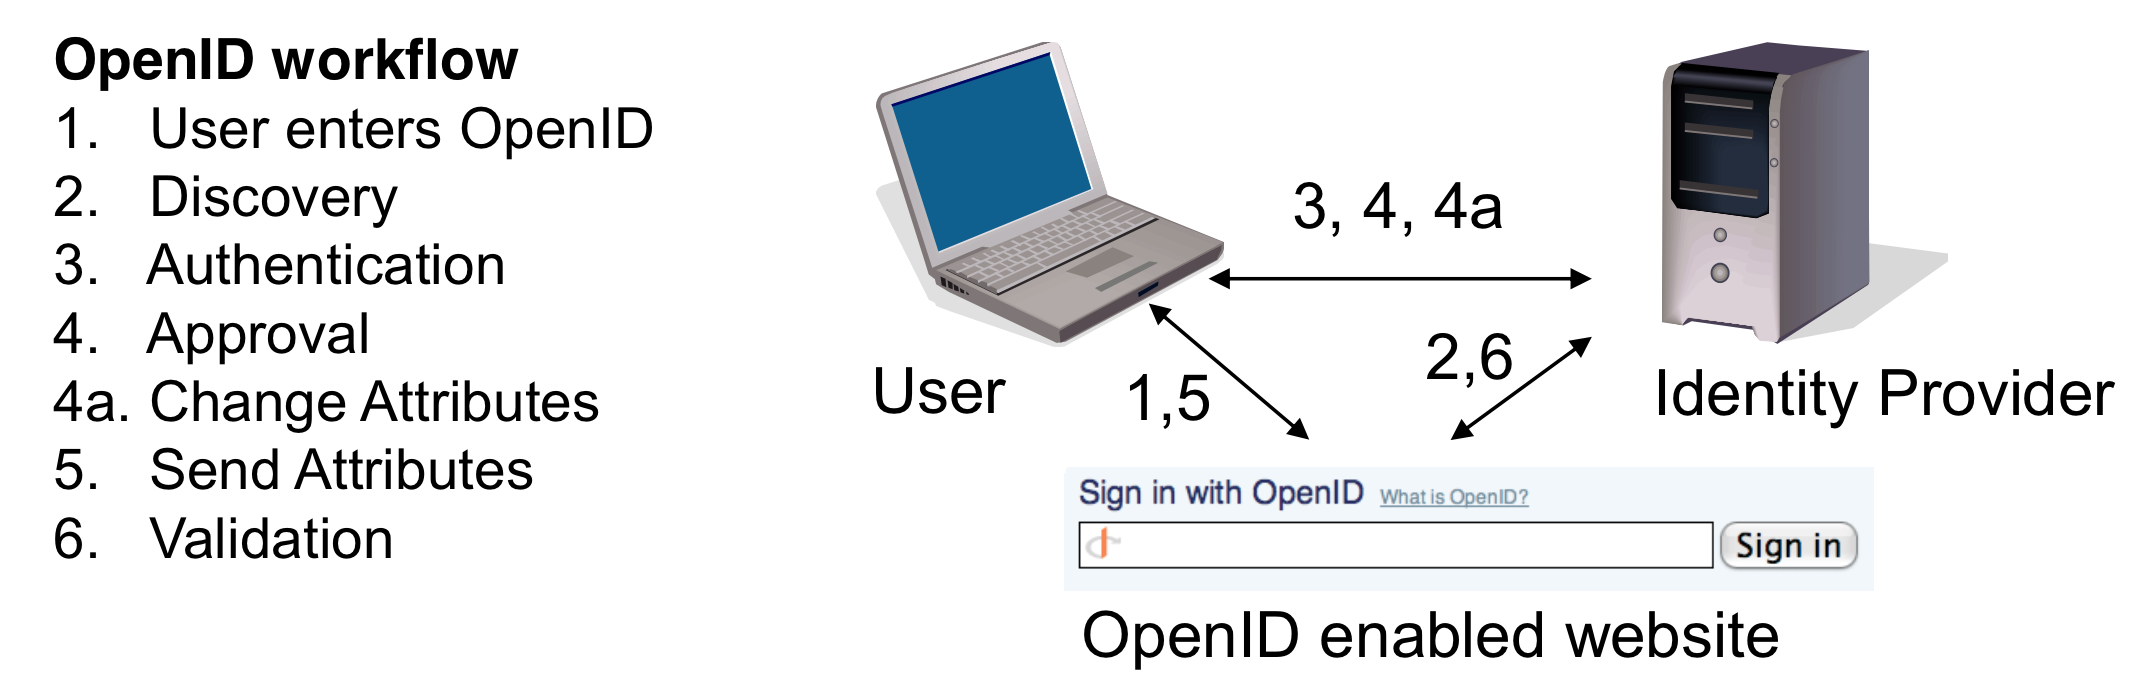
\includegraphics[width=\columnwidth]{img/OpenID.png}
  }
  \sectionbox{
  \subsubsection{OAuth}
    A web user (resource owner) grants a
    printing service (client) access to her protected photos stored at a photo sharing service (resource server), without sharing her username and password with the printing service.
    Instead, she authenticates directly with a server trusted by the photo sharing service (authorization server) which issues the printing service delegation-specific credentials (access token).

    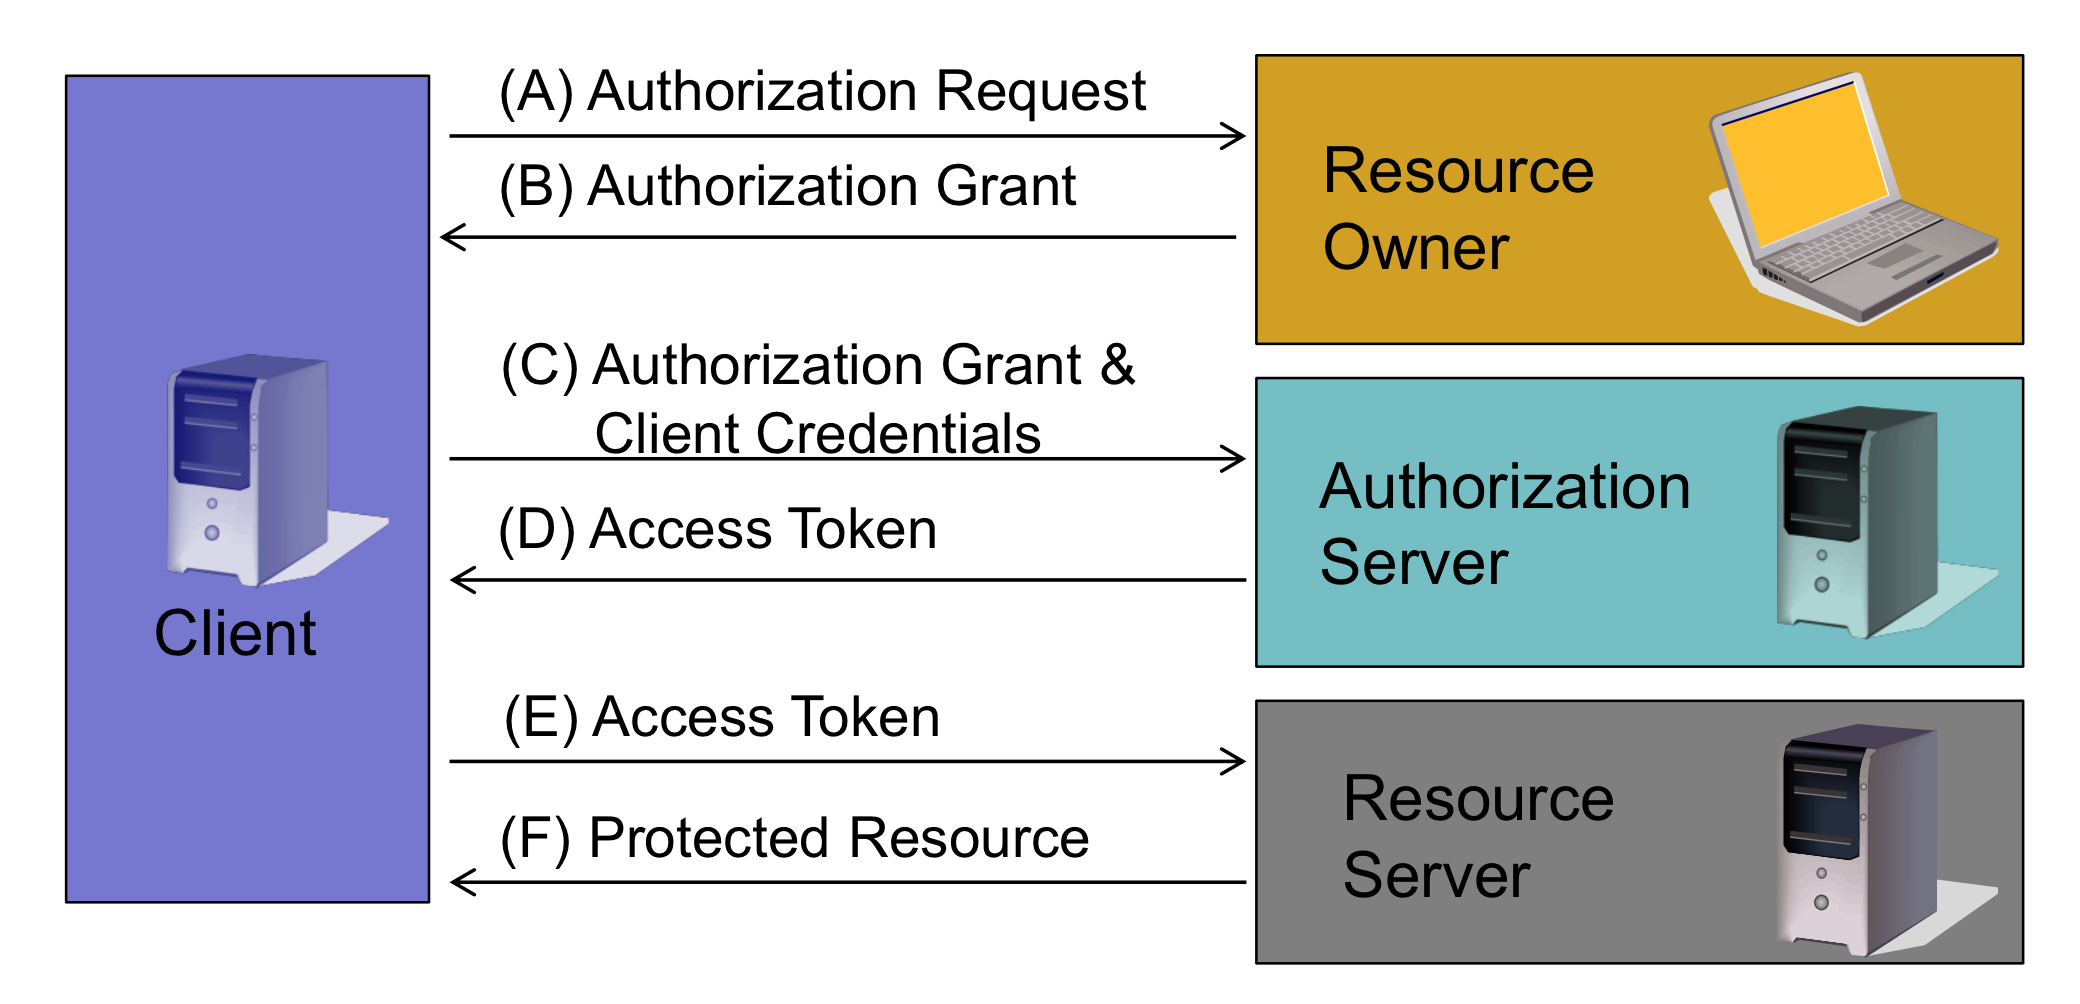
\includegraphics[width=\columnwidth]{img/OAuth.png}

    (A) Client requests authorisation from the resource owner or authorization server. \\
    (B) Client receives an authorisation grant by the resource owner. Authorization grant type depends on the method used by the client and supported by the authorisation server to obtain it. \\
    (C) Client requests an access token by authenticating with the authorization server using its client credentials (prearranged between the client and authorization server) and presenting the authorization grant. \\
    (D) Authorisation server validates  client credentials and the authorisation grant, and if valid issues an access token.\\
    (E) Client requests protected resource from the resource server. Authentication by access token.\\
    (F) Resource server validates the access token \ra valid \ra serves request\\
  }
  \sectionbox{
  \subsubsection{3D Secure}
    A protocol used widely to authenticate online card transactions.

    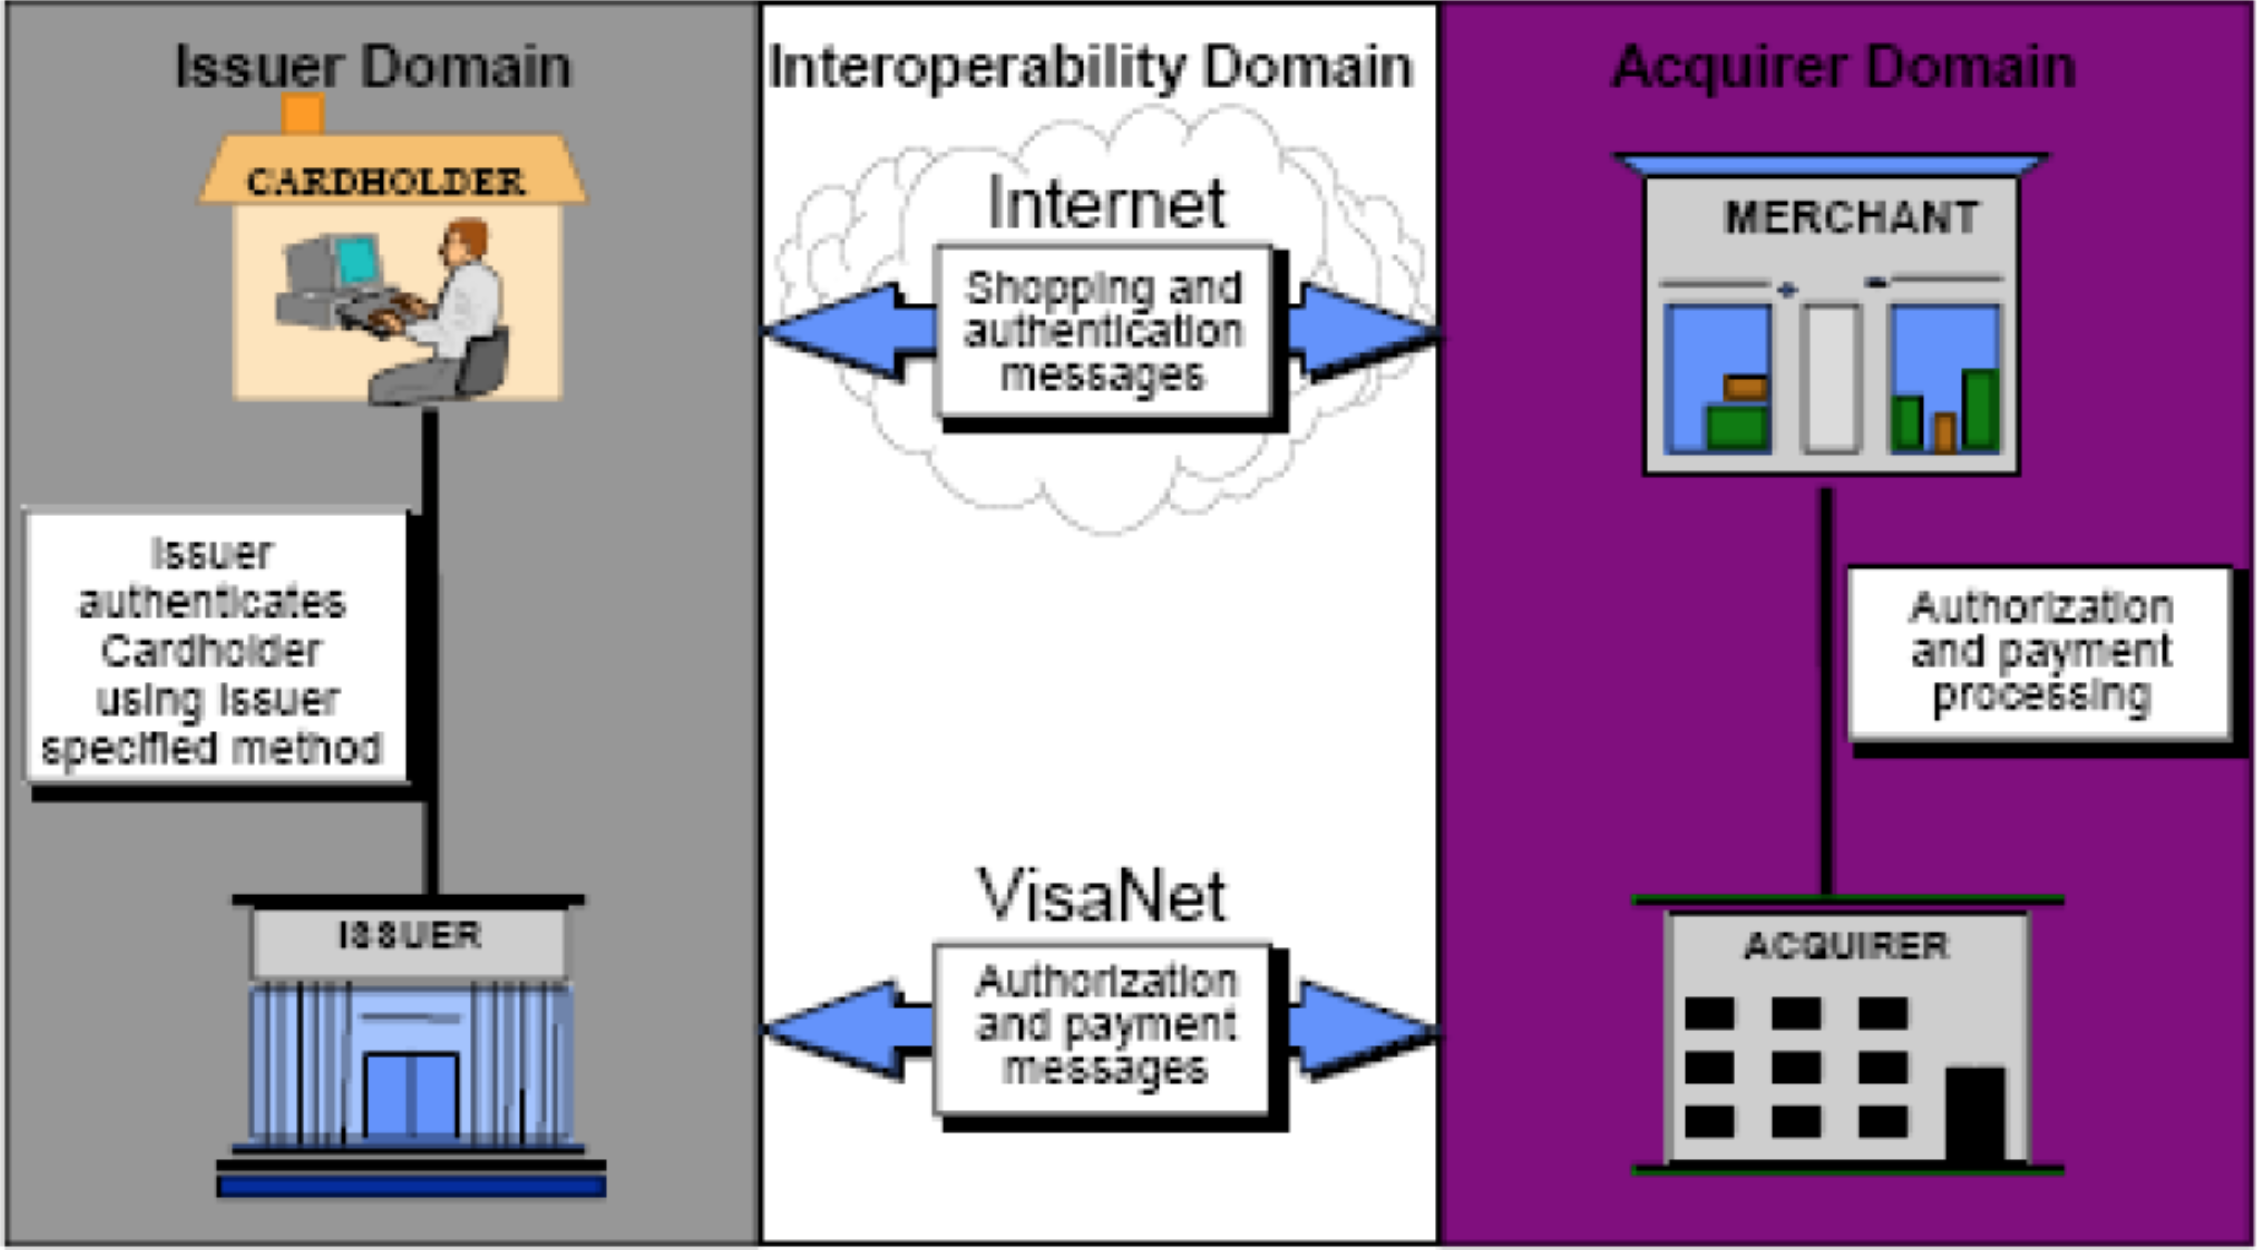
\includegraphics[width=\columnwidth]{img/3DSecure.png}
    After entering payment card details on merchant site:
    \begin{itemize}
    \item 3D Secure pops up a password entry form to a bank customer
    \item customer enters a password and, if it was correct,
    \item customer is returned to the merchant website to complete the
    transaction and
    \item the merchant gets an authorisation code to submit to his bank
    \end{itemize}

    \textbf{Problems:} Pop-Up blockers, Activation during shopping, SLL verification not visible, liability shift, weak bank authentication, no password reset procedure, privacy issues\\
  }
  \sectionbox{
  \subsubsection{802.1x : Port-Based Network Access Control}
    Client-server based access control protocol that restricts unauthorised devices from connecting to a (W)LAN through publicly accessible ports.

    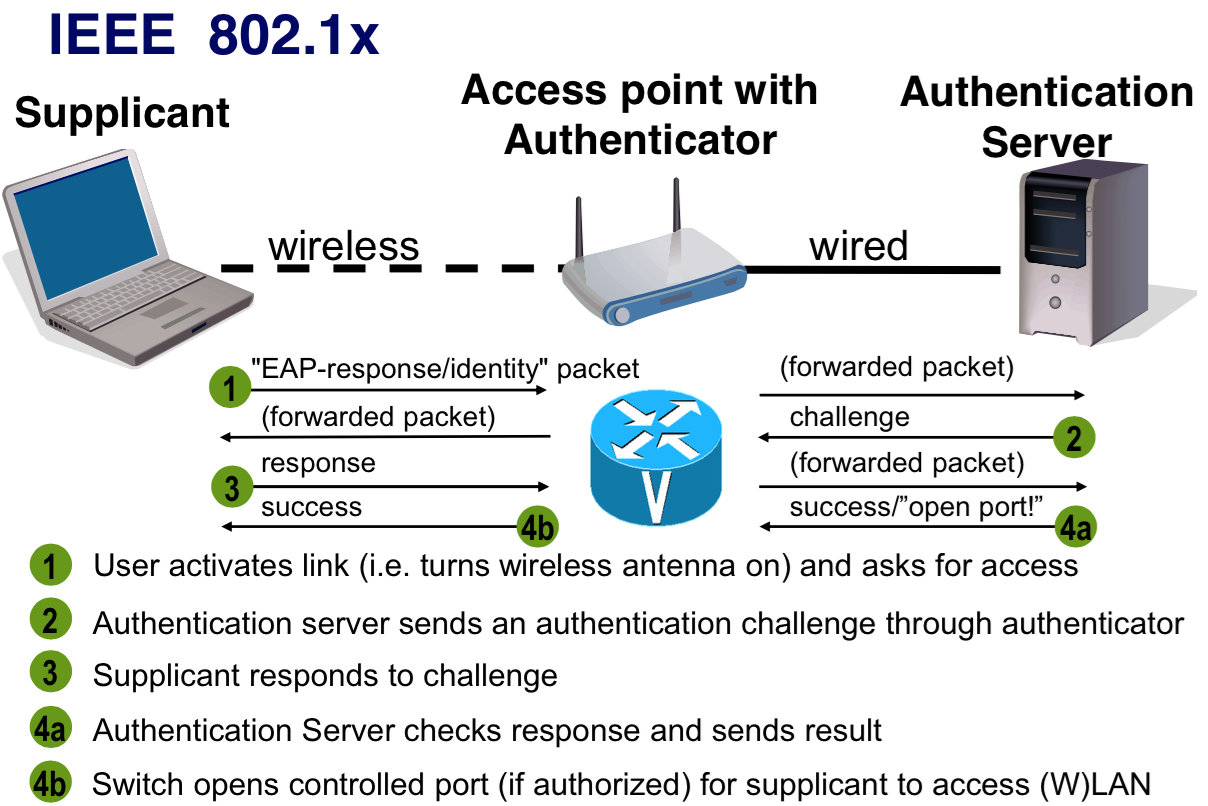
\includegraphics[width=\columnwidth]{img/8021x.png}

    \textbf{EAP} (Extensible Authentication Protocol): Authentication framework on the data link layer supporting multiple methods (MD5, OTP, TLS, TTLS) without requiring an IP.

    \textbf{Identity and Security}: Authentication (Who?) , Authorisation (What?) , Access Control, Policy enforcement

    \textbf{Benefits:} Standard based technology, control at link layer, interoperating wifi and wired, centralised user administration

    \textbf{Drawbacks:} Authenticator authentication, Man-in-the-middle, session hijacking
  }

  \sectionbox{
  \subsection{Anonymization}
    \textbf{Levels of Anonymity:} Identity (principal known), Pseudonymity (indirectly kown as pseudonym), anonymity (part of anonymity set but within no distinguishing)

    \textbf{Pseudonyms:} public (\ra identification), non-public (\ra pseudonymity), unlinkable (\ra anonymity)

    \textbf{Use cases:} \\
    physical: feedback, voting, whistleblowing, censorship \\
    digital: digital cash, digital voting, illegal activities

    \textbf{Oninon routing: } Data is encapsulated multiple times and only the next hop is known to each node

    \textbf{Mixnet:} proxy handles messages in batches (transformed and premutated) \Ra unlinkablity of incoming and outgoing messages

    \textbf{Attacks:} Traceback (break systems on path), Collusion (bad nodes), Traffic analysis (tagging with bit errors, replay messages - defense: heartbeats, traffic shaping, padding) , Logging (???)
  }


\section{Firewalls, IDS and NAT Traversal}
  \sectionbox{
  \subsection{Firewalls}
    Hardware or software device which is configured to permit, deny or proxy data through a computer network with different levels of trust. The configuration is called \emph{policy}.

    \textbf{Types:} simple packet filter, stateful filter, application layer proxy

    \textbf{Rules:} Filtering (outgoing (egress), incoming), Default (accept, reject), Deny (Drop, Reject), Addressing Transparency (firewall and network fingerprinting)
    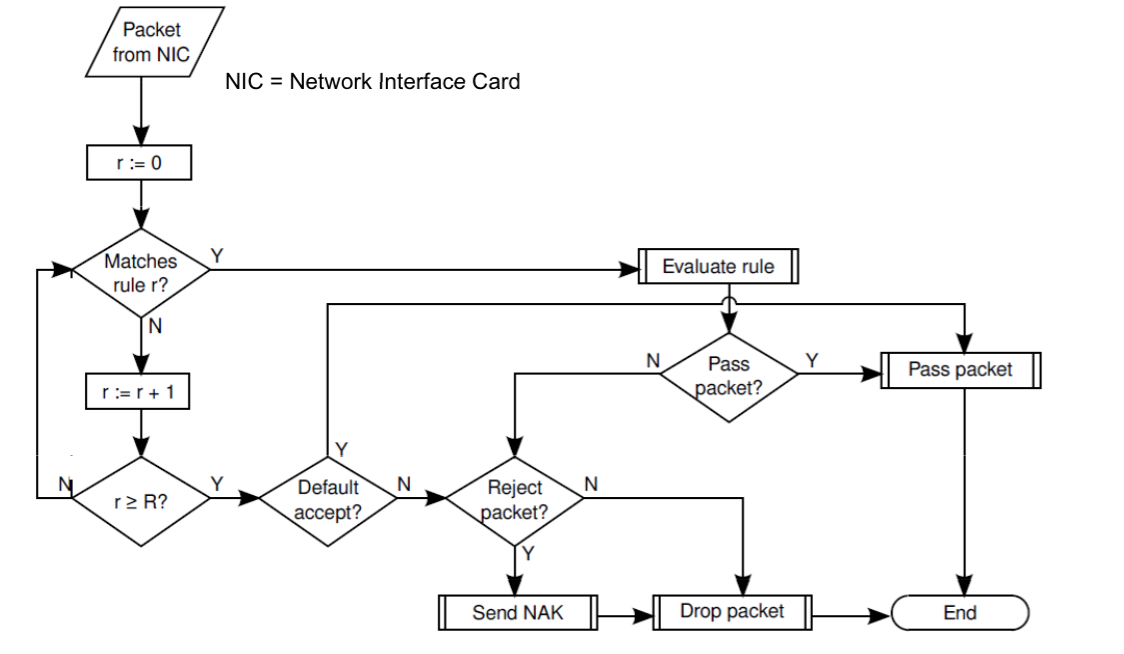
\includegraphics[width=\columnwidth]{img/firewallrule.png}

    \subsubsection{Stateless Firewall}
    Functionality: examine on network layer, decision based on header

    Pro: application independent, good performance

    Cons: no state or application context

    \subsubsection{Stateful Firewall}
    keeps track of state. Decision based on \emph{session state}

    Pro: more powerful

    Cons: no state for UDP, host vs. firewall state, state explosion

    \subsubsection{Application Layer Firewall}
    take application state into account

    Pro: application aware

    Cons: many application protocols, performance

    \subsubsection{Web Application Firewall}
    protects web-based applications from malicious requests (often reverse proxy)

    Filtering: signatures, black/whitelisting
    } \sectionbox {
    \subsection{Firewall Attack techniques}
    \begin{itemize}
    \item IP source spoofing
    \item artificial fragmentation
    \item vulnerabilities
    \item Denial of Service (state explosion)
    \item Tunnelling/Covert channel (ICMP, DNS, \ldots)
    \end{itemize}
  } \sectionbox {
  \subsection{Firewall detection}
    Port scanning: traceroute, src IP of response

    TTL:  let expire TTL one hop past firewall
    } \sectionbox {
    \subsection{Oranizational challenges}
    \begin{itemize}
      \item Large rulesets
      \item Big Organisations
      \item Conflict: Networking vs. security staff
    \end{itemize}
  } \sectionbox {
  \subsection{IP Tables}
    Netfilter rule:
    iptables -A INPUT -i eth0 -m state --state ESTABLISHED, RELATED -j ACCEPT

    Iptables rule:  iptables -A INPUT -p tcp -s 0/0 -d 0/0 --destination-port 80 --syn -j ACCEPT
    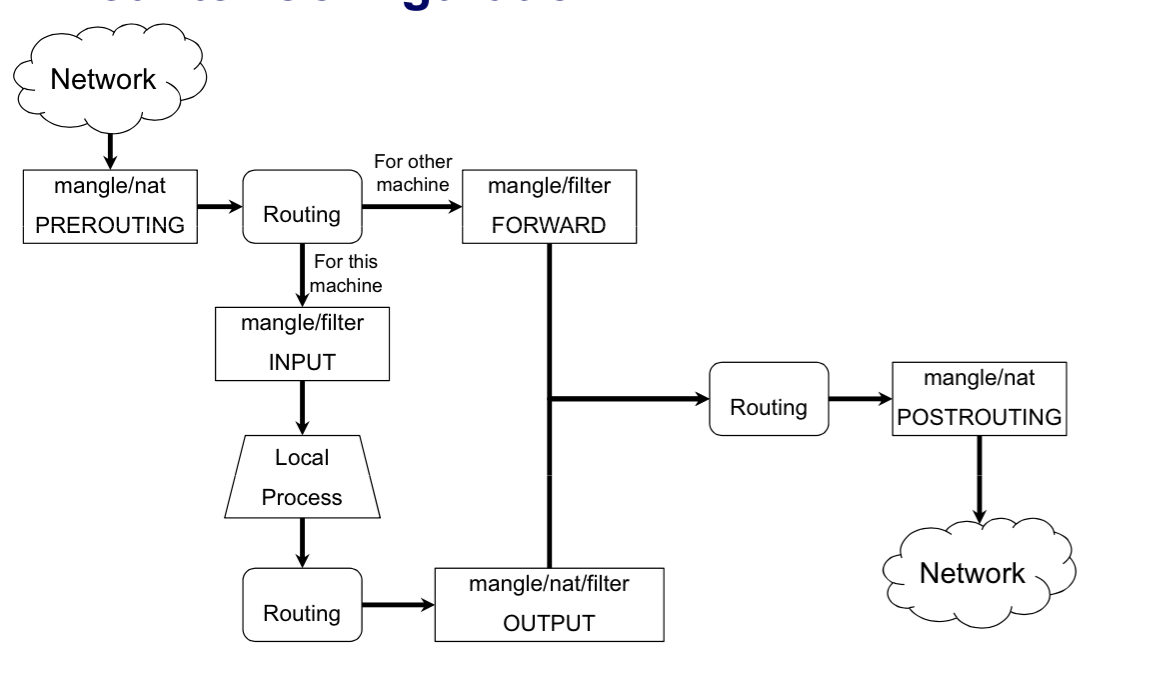
\includegraphics[width=\columnwidth]{img/netfilter.png}
   }
   \sectionbox {
   \subsection{NAT (Network Address Translation)}
    One-to-many (multiple hosts on private network using the same public IP address). IP Address rewriting.

    \textbf{Benefits}: Saves address space + Prevents malicious activity from outside (Don't use it for security as a Firewall)

    \textbf{Drawbacks}: no end-to-end connectivity + P2P and IPSec don't work

    \textbf{NAPT} = Network Address and Port Translation (Most used one)

    \subsubsection{NAT UDP Hole Punching (using RDV server)}

    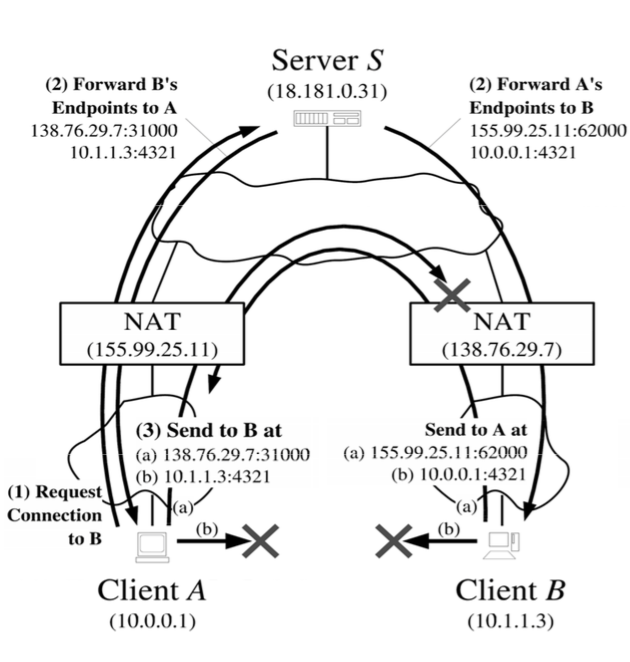
\includegraphics[width=\columnwidth]{img/nathole.png}
  }
  \sectionbox{
  \subsection{Intrustion Detection and Prevention Systems}
    try to detect intrusions on the network by comparing to attack signatures. Block traffic after detection.

    \subsubsection{Classification}
    \textbf{Object of observation:}

    Packet:

    Flow: scalabilty (+), encryption (+), not content-based (-)

    \textbf{Point of observation:}

    Host: hard deployment (-), context information (+), one sensore per machine (+)

    Network: easy deployment (+), multiple machines (+), unknown machines(-), preformance (-)

    \textbf{Method of observation:}

    Signature: precision (+), not detecting unknown attacks (-)

    Behavior: unknown attacks (+), difficult to find ground truth (-), false positives (-)

    \subsubsection{Challenges}
    \begin{itemize}
    \item false alarms
    \item high network speeds
    \item sensor management and signature distribution
    \item policy management
    \item manpower
    \end{itemize}

    \subsubsection{Attacks}
    \begin{itemize}
    \item Flooding / resource exhaustion
    \item algorithmic Complexity Attacks (e.g. on hash table)

    \end{itemize}
  }


\section{The Domain Name System Security}
  \sectionbox{
  \subsection{DNS}
    \emphbox{DNS is a global, distributed, robust system for name to IP address resolution}

    DNS is the glue of the internet: Nearly all activities start with a DNS lookup (Orginally: no security considerations)

    Design:
    \begin{itemize}
    \item Client-Server application
    \item Hierarchical System
    \item Use UDP on port 53
    \end{itemize}

    \textbf{Zone:} Collection of hostnames/IP pairs managed together

    \textbf{Nameserver (authoritative): } Server that answers DNS queries (Responsible DNS Server for each zone)

    \textbf{Resolver:} Client part of DNS that resolves domain names

    \textbf{Recursive name server:}  Answers queries for all zones

    \textbf{Stub resolver:} Forwards request to recursive name server (typically used by end-hosts)

    \textbf{Caching:} Reduces overhead. Lifetime controlled by TTL
  }
  \sectionbox{
  \subsection{Attacks on DNS}
    \subsubsection{Denial of Service on DNS}
    Targeting the 13 DNS root servers which are a bottleneck resource. However over-provisioning (13 clusters) + Anycast (\textgreater 500) (1 address to multiple potential receivers) prevents most attacks.

    \subsubsection{Account-Takeover}
    Attacking the web interfaces of registrars and try to enter malicious name servers.

    \subsubsection{Manipulate local DNS settings}
    \begin{itemize}
    \item Manipulate local host configurations (access to the local machine nescessary)
    \item Spoof DHCP replies (access to LAN nescessary) \ra countermeasure: authentication for DHCP messages
    \item Set up Malicious DHCP server that is faster than the valid one
    \end{itemize}

    \subsubsection{Manipulate DNS lookup process}

    \textbf{Bailiwick Checking:} Is the server authorized to respond to DNS requests for the domain.

    \textbf{Weak authentication:} Port, TXID, Query string - first good answer wins

    3 possible answers to DNS queries:
    \begin{itemize}
      \item Here is your answer
      \item go away
      \item I don't know ask \ldots
    \end{itemize}


    \subsubsection{The Kaminsky Attack}
    \begin{itemize}
    \item Inject query on the client \textit{\$Random}.www.bank.com
    \item reply multiple times  (TXID 0-200)
    \item Send name server redirections
    \end{itemize}
    $\Ra$ Fix: Source Port Randomization. Chance: $65536 \cdot (65536 - 1024)$ to 1
  }

  \sectionbox{
  \subsection{DNSSEC}
    Provides:
    \begin{itemize}
      \item Authenticity
      \item Integrity
      \item Backward compatibility
    \end{itemize}

    Drawbacks
    \begin{itemize}
      \item No confidentiality
      \item No protection against DoS
      \item Must be installed from a trusted source
    \end{itemize}

    All records are signed: Key pairs for each zone $\ra$ Integrity

    Chain of trust $\ra$ Authenticity
  }

\section{Availability and Denial of Service}
  \sectionbox{
  \subsection{System Level Agreements (SLA)}
    \begin{tabular}{ l | l | l }
      Level & Percentage & Downtime \\ \hline
      Two-nines & 99 & 3.5 days \\
      Three-nines & 99.9 & 9 hours \\
      Four-nines & 99.99 & 53 minutes \\
      Five-nines & 99.999 & 5 minutes \\
      Six-nines & 99.9999 & 31 seconds \\
    \end{tabular}

    How to achieve 99.999:
    \begin{itemize}
      \item High Redundancy + Fast Failover (Quick Change)
      \item Failure Resilience
      \item Over Provisioning
      \item Backup and Fast Recovery
    \end{itemize}
  }
  \sectionbox{
    \subsection{Denial of service}
    DoS: Resource starvation of CPU, Storage, Network

    Attacks:
    \begin{itemize}
      \item SYN-Flood: Spam Server with TCP SYNs $\rightarrow$ needs to keep state $\rightarrow$ Solution: Choose carefully constructed initial sequence number (crypto based)
      \item Compression Bomb
      \item Source Spoofing/Reflector Attack
      \item Mail Bounce: reply-to: @victim.com, To: and multiple Bcc: @target.com
      \item DNS Amplification: Send small request to recursive servers with spoofed source
    \end{itemize}
  }
  \sectionbox{
  \subsection{Dos Countermeasures}
    Prevention
    \begin{itemize}
      \item secure systems (e.g. prevent machine compromise to build bot
      nets by patching, IDS/IPS, firewall etc.)
      \item secure protocols (e.g. prevent IP spoofing, use TCP SYN
      cookies, HashCash: add client CPU cycles)
      \item resource accounting (server commits resources only to
      authenticated/trustworthy clients)
      \item resource multiplication (resource over provisioning for the case
      of an attack)
      \item late resource binding (bind resources as late as possible)
    \end{itemize}

    Reaction:
    \begin{itemize}
      \item detect (using pattern, anomaly, third party)
      \item react (rate-limit, filter, reconfigure, identify agents)
    \end{itemize}
  }

\section{Secure Channels: Principles, VPN, SSH}

  \sectionbox{
  \subsection{Security by Layer of the TCP/IP Model}
  Properties of a secure channel: secure = authentic and confidential

  \subsubsection{Security at Link Layer}
  \begin{itemize}
  \item All traffic over a specific Link
  \item Often implemented in hardware
  \end{itemize}

  Pro: Speed, Seamless

  Drawbacks: every link seperately, trust in link operator

  \subsubsection{Security at Internet Layer}
  secure traffic over multiple links between end points (e.g. IPSec)

  Pro: seamless security to above layers, IPSec part of IPv6 + IPv4

  Cons: complex configuration, tunnel mode encrypts only part of a route


  \subsubsection{Security at Transport Layer}
  e.g. TLS/SSL, SSH

  implemented in end-hosts

  Pro: can be added to existing apps, portable and easy configuration

  Cons (of TLS): protocol specific, application must be TLS/SSL aware


  \subsubsection{Security at Application Layer}

  implemented in end hosts (PGP, S/MIME, Skype, \ldots)

  Pros: extend app without involving OS, applications understand data

  Cons: seperate security for each app
  }

  \sectionbox{
  \subsection{VPN}
  connect networks or machines over an existing network

  \subsubsection{Tunnel mode}
  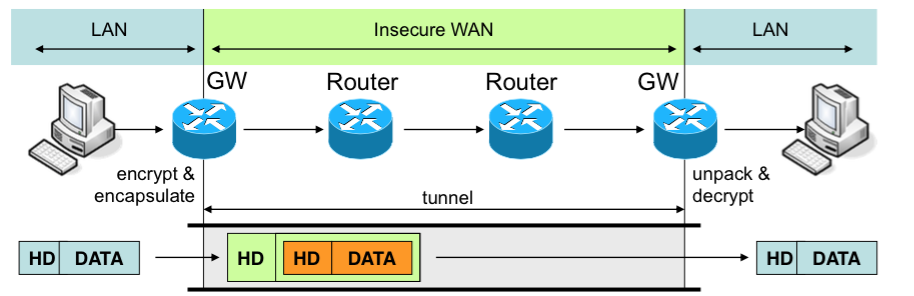
\includegraphics[width=\columnwidth]{img/vpntunnel.png}
  \begin{itemize}
  \item encrypt and authenticate orgininal IP packet
  \item transport htis as payload in new IP packet
  \end{itemize}
  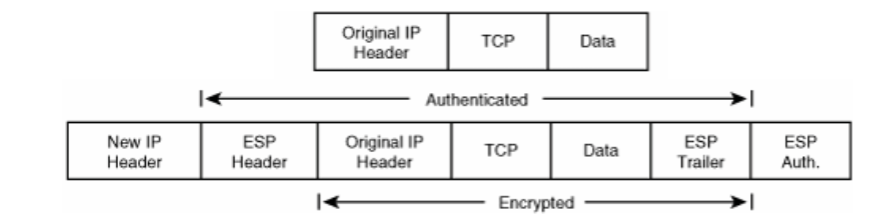
\includegraphics[width=\columnwidth]{img/vpntunnel2.png}
  \subsubsection{Transport mode}
  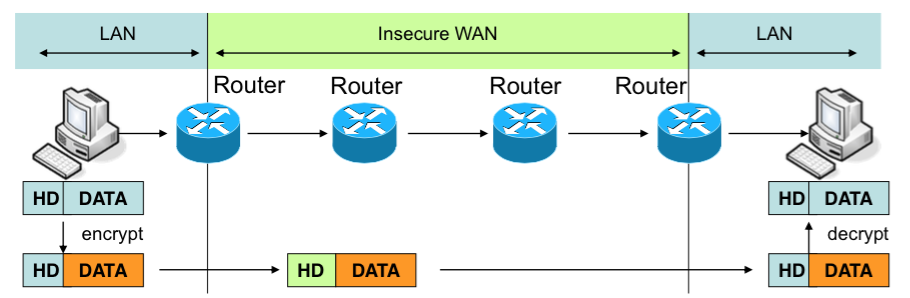
\includegraphics[width=\columnwidth]{img/vpntransport.png}
  \begin{itemize}
  \item end-to-end communication between hosts
  \item encrypt and authenticate payload only
  \end{itemize}
  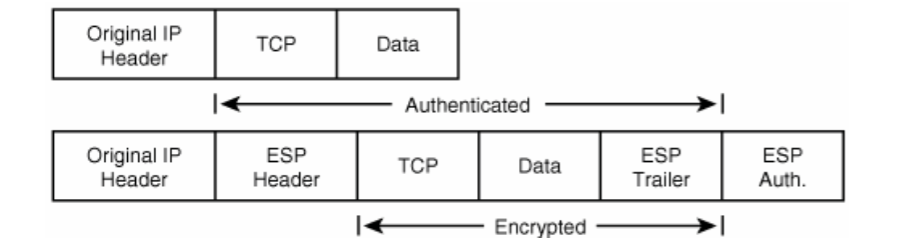
\includegraphics[width=\columnwidth]{img/vpntransport2.png}

  \begin{itemize}
  \item encryption
  \item randomized IVs
  \item replay protection
  \item authentication (HMAC)
  \end{itemize}

  \subsubsection{Security Association (SA)}
  A Security Association (SA) is the establishment of shared security attributes between two network entities to support secure communication. An SA may include attributes such as: cryptographic algorithm and mode; traffic encryption key; and parameters for the network data to be passed over the connection.
  } \sectionbox{
  \subsection{Message Authentication Code (MAC)}
  Provide data and integrity
  \begin{itemize}
  \item message not modigied in transit
  \item source is authentic
  \item not delayed
  \item sequence order
  \end{itemize}

  MAC (K, M) = DES (K, M) take last 32 bits

  \subsubsection*{HMAC (Mac with Hash functions)}
  \begin{itemize}
  \item use hash functions (MD5, SHA)
  \item faster
  \item easy availible
  \end{itemize}

  HMAC (K, M) = H(K' xor opad | H (K' xor ipad | M))


  } \sectionbox{
  \subsection{SSH}
  standard for remote login and encrypted file transfer

  \subsubsection{Protocols}
  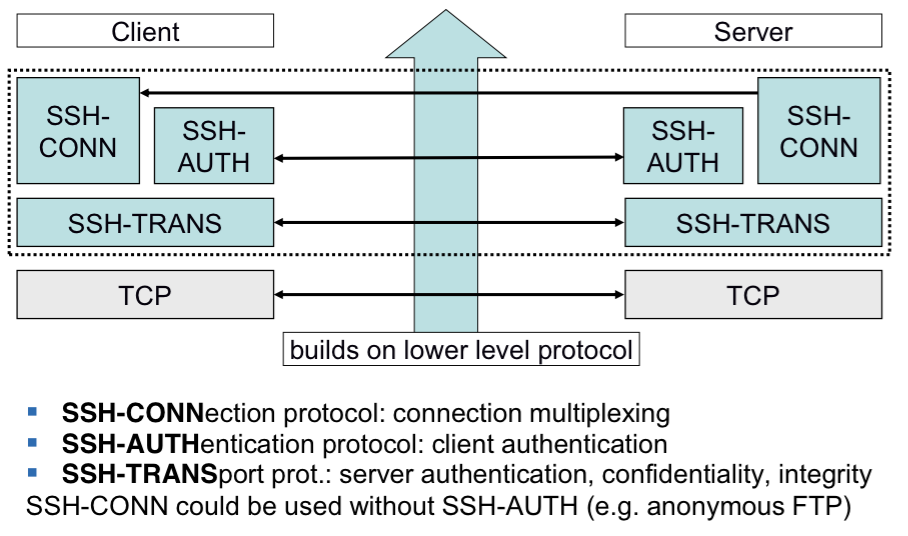
\includegraphics[width=\columnwidth]{img/sshproto.png}

  \subsubsection{SSH-Trans}
  \begin{itemize}
  \item algorithm negotiation
  \item session key exchange (e.g. Diffie-Hellman)
  \item session id
  \item server authentication
  \item encryption, integrity, data compression
  \end{itemize}

  \subsubsection{SSH-Auth}
  \begin{itemize}
  \item authenticates the client with multiple auth mechanisms
  \item defines format of auth-requests (Username, Method name, Service name)
  \end{itemize}

  \subsubsection{SSH-Conn}
  \begin{itemize}
  \item multiplexing multiple steams
  \item port forwarding
  \item compression handling
  \item interactive and non-interactive sessions
  \end{itemize}


  \subsubsection{Attacks}
  \begin{itemize}
  \item password cracking
  \item traffic analysis
  \end{itemize}
  }

\section{TLS (Transport Layer Security)}
  \sectionbox{
    \begin{itemize}
      \item Session or Application layer (OSI model)
      \item SSL (Secure Socket Layer) = predecessor of TLS
      \item SSLv3 and TLS almost same except some crypto algo.
    \end{itemize}
  }

\sectionbox{
\subsection{Diffie-Hellman Key Exchange (DH)}
  \begin{itemize}
    \item \textbf{Public	values}:	large	prime	$p$,	generator	$g$
    \item \textbf{Secret values}: Alice	has	$a$,	Bob	has $b$
    \item Alice	$\ra$ Bob:	$A = g^a \pmod{p}$
    \item Bob	$\ra$ Alice:	$B = g^b \pmod{p}$
    \item Bob computes	$A^b	\pmod{p}=	g^{ab}\pmod{p}$
    \item Alice	computes $(B)^a	\pmod{p}=	g^{ab}\pmod{p}$
    \item Alice and Bob have now a shared secret $g^{ab}\pmod{p}$
    \item Eve	cannot	compute	$g^{ab}	\pmod{p}$
  \end{itemize}
}

\sectionbox{
\subsection{Generation of Crypto Parameters}
  \textbf{Master Secret}(MS) created from pre-master secret(PS), client random(CR), server random(SR): MS = $h('A') || h('BB') || h('CCC')$

  with $h(X) = MD5(PS || SHA(X || PS || CR || SR ))$

  \textbf{Key materials} pairs client \& server: MAC key, write key and write IV \texttt{key\_block} = $h_2('A') || h_2('BB') || h_2('CCC') || \cdots$

  with $h_2(X) = MD5(MS || SHA(X || MS || CR || SR ))$
  \begin{itemize}
    \item \texttt{key\_block} is the concatenation of the 6 keys
    \item Nb of round depends on size of keys $\ra$ MD5 = 16 bytes per round
    \item MS $\simeq$ pseudorandom seed value and CR and SR $\simeq$ salt values
  \end{itemize}
}

  \sectionbox{
  \subsection{Key Exchange Methods}
  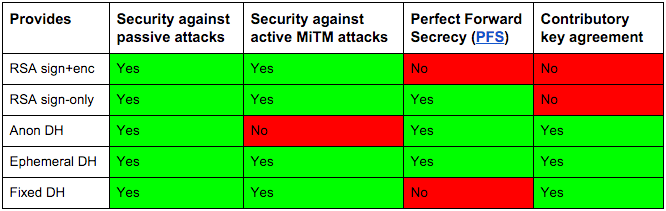
\includegraphics[width=\columnwidth]{img/Key-Exchange-Algorithms.png}

  \begin{itemize}
    \item \textbf{Contributory Key Agreement} = Both parties contribute to session key, no party can fully determine session key.
    \item \textbf{Perfect Forward Secrecy} = knowing long-term private key does not reveal session key.
  \end{itemize}

  \subsubsection{RSA}
    Pre-master secret(PMS)= 48-bytes (2 protocol version + 46 random)\\
    \textbf{sign+enc}: client generates pre-master and encrypts it with $PU_{server}$.
    \begin{itemize}
      \item No \texttt{server\_key\_exchange} msg needed in phase 2
      \item Always same public/private keys used $\Ra$ no PFS $\Ra$ Not recommended
    \end{itemize}

    \textbf{sign-only}: Server RSA keys used for signature only
    \begin{itemize}
      \item Server creates temporary RSA keys, signs them with $PR_{server}$ and use \texttt{server\_key\_exchange} to send them
      \item PMS encrypted with temporary server public key
    \end{itemize}

  \subsubsection{Diffie-Hellman}
    \textbf{Anonymous DH}: No authentication of client nor server
    \begin{itemize}
      \item \texttt{server\_key\_exchange}: DH public values + server public DH key
      \item \texttt{client\_key\_exchange}: client public DH key
      \item Vulnerable to MitM attacks
    \end{itemize}

    \textbf{Ephemeral DH}: create ephemeral (one-time) secret keys
    \begin{itemize}
      \item \texttt{server\_key\_exchange}: DH public values + server public DH key + signature of those parameters
      \item \texttt{client\_key\_exchange}: client public DH key
      \item Don't provide authentication but signing values with RSA does.
      \item Most commonly used
    \end{itemize}

    \textbf{Fixed DH} : DH public values + server public values are fixed
    \begin{itemize}
      \item All DH parameters in server certificate signed by CA $\Ra$ no need of \texttt{server\_key\_exchange}
      \item server can asked client to be authenticated with \texttt{certificate\_request}
      \item Rarely used
    \end{itemize}
  }

  \sectionbox{
  \subsection{Attacks against SSL/TLS}
    \subsubsection{Dumbing Down}
      \begin{itemize}
        \item attacker forces to use old breakable algo. for communication (using the \texttt{ciphersuite})
        \item only DOS except with anon DH where it can become real MitM
      \end{itemize}

    \subsubsection{Attacks against CAs}
      \begin{itemize}
        \item Attacks against CA to get false certificates signed
        \item any CA can issue certs for any domain (weakest link)
        \item 2010: Stuxnet signed itself 2 compromised Taiwan CAs' private keys
        \item 2011: Comodo was duped into creating certificates for Google sites
      \end{itemize}

    \subsubsection{BEAST}
      \begin{itemize}
        \item Vulnerability in the Initialization Vector (IV) of the CBC mode of AES
        \item  MitM can read msg by encrypting it multiple times
        \item mitigated in TLS1.1 and above
      \end{itemize}

    \subsubsection{Assumption for Secure TLS}
      \begin{itemize}
        \item CA, Crypto, Browser, User
        \item if a single assumption does not hold $\Ra$ TLS not secure
      \end{itemize}
  }

  \sectionbox{
  \subsection{Handshake Protocol}
    \subsubsection{Phase 1: Establish Security Capabilities (hello\_messages)}
      \begin{enumerate}
        \item C $\ra$ S: \texttt{client\_hello}
        \begin{itemize}
          \item \textbf{version}: highest supported version.
          \item \textbf{ciphersuite}: Supported ciphers listed in $\searrow$ order of pref.\\
          := Key exchange algo. + Cipher algo. (RC4, AES, 3DES…) + MAC algo. (MD5 or SHA-1) + \dots
          \item \textbf{random}: 32-bit timestamp + 28 bytes random $\Ra$ prevent replay
          \item \textbf{compression}: list of compression methods
          \item \textbf{SessionID}: update (value=which session) or create (value=0)
        \end{itemize}
        \item S $\ra$ C: \texttt{server\_hello}: Reply to every param.
      \end{enumerate}

    \subsubsection{Phase 2: Server Authentication and Key Exchange}
      \begin{enumerate}
        \item S $\ra$ C: \texttt{certificate}*: except for Anon DH, contains public DH param if DH fixed used
        \item S $\ra$ C: \texttt{server\_key\_exchange}*: required for Anon DH, Ephemeral DH, RSA sign-only
        \item S $\ra$ C: \texttt{certificate\_request}*: request types of cert. from client
        \item S $\ra$ C: \texttt{server\_hello\_done}: no param. + wait for client response
      \end{enumerate}

    \subsubsection{Phase 3: Client Authentication and Key Exchange}
      Client should verify server certificate (if required) + server parameters
      \begin{enumerate}
          \item C $\ra$ S: \texttt{certificate}*: client cert. or \texttt{no\_certificate} alert
          \item C $\ra$ S: \texttt{client\_key\_exchange}
          \begin{itemize}
            \item \textbf{RSA}: 48 bytes pre-master secret encrypted with server’s public key
            \item \textbf{DH}: client public DH values
          \end{itemize}
          \item C $\ra$ S: \texttt{certificate\_verify}*: hash of master secret + previous msgs encrypted with client private key (except fixed DH)
      \end{enumerate}

    \subsubsection{Phase 4: Finish}
    \begin{enumerate}
      \item C $\ra$ S: \texttt{change\_cipher\_spec}: Send 1 byte to confirm encryption.
      \item C $\ra$ S: \texttt{finished}: hash( master\_secret $||$ pad2 $||$ hash( handshake\_messages $||$ Sender $||$ master\_secret $||$ pad1 ))
      \begin{itemize}
        \item once with MD5(...) and once with SAH-1(...)
        \item \texttt{handshake\_messages} = all messages until now
      \end{itemize}
      \item S $\ra$ C: \texttt{change\_cipher\_spec}: server confirm encryption too
      \item S $\ra$ C: \texttt{finished} 1st encrypted msg = hash of all previous msg
    \end{enumerate}

  \textit{* = optional or situation-dependent messages that are not always sent}
  }

  \section{Certificates and PKI (Public Key Infrastructure)}

    \sectionbox{
    \subsection{Public-Key Certificates}
      Certificate = (public key + id of key owner)*signed by a trusted 3rd party
      \begin{enumerate}
        \item All can determine name + public key of the certificate’s owner
        \item All can verify signature of CA
        \item Only CA can create and update certificates
        \item All can verify the currency of the certificate
      \end{enumerate}

      \subsubsection{Revocation of Certificates}
      \begin{enumerate}
        \item User’s private key is assumed to be compromised
        \item User is no longer certified by this CA
        \item CA’s certificate is assumed to be compromised.
      \end{enumerate}
      \textbf{CRL}(Certificates Revocation List): listing of all the revocated certifactes by a CA.
    }

    \sectionbox{
    \subsection{OCSP (Online Certificate Status Protocol)}
      \begin{itemize}
        \item Small bandwidth needs $\Ra$ Real-time checks
        \item Privacy issues $\leftarrow$ OCSP responder can track users
        \item OCSP servers need to answer every client request (no cache)
        \item if connection fails, client has to make the choice on its own
        \item OCSP stapling: certificate owner give OCSP response with its certificate
      \end{itemize}
    }

    \sectionbox{
    \subsection{GL: Certificate Transparency}
      Protocol for publicly logging the certificates activity.\\
      $Ra$ augment chain-of-trust for the entire SSL certificate system.
      \begin{itemize}
        \item \textbf{Logs}: log cryptographically secured in a Merkle hash tree
        \item \textbf{Monitors}: watch for suspicious or missing certificates in logs
        \item \textbf{Auditors} : verify the overall integrity of logs
      \end{itemize}

      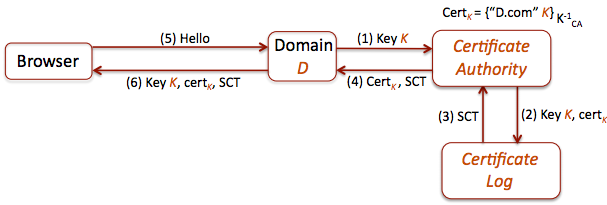
\includegraphics[width=\columnwidth]{img/CT.png}

      \textbf{Benefits:} Gradual rollout + Minimal impact on existing infrastructure

      \textbf{Disadvantages:} MitM, no support revocation, still need to contact log to verify
    }

    \sectionbox{
    \subsection{AKI (Accountable Key Infrastructure)}
      \begin{itemize}
        \item New public-key validation infra. to reduce lvl of trust in CAs
        \item Distribute trust $\ra$ no single point of failure
        \item support revocation and update of certificates
        \item Based on integrity tree (Efficient representation of the current state of all domains)
      \end{itemize}
    }

\section{Web Application Security}
  \sectionbox{
  \subsection{Top 10 Application Security Flaws}
    \begin{tabular}{ l | l }
      A1 & Injection (SQLi, LDAP, XPATH, OS Command)\\
      \hline
      A2 & Broken Authentication and Session Management\\
      \hline
      A3 & Cross-Site Scripting (XSS)\\
      \hline
      A4 & Insecure Direct Object References\\
      \hline
      A5 & Security Misconfiguration\\
      \hline
      A6 & Sensitive Data Exposure\\
      \hline
      A7 & Missing Function Level Access Control\\
      \hline
      A8 & Cross-Site Request Forgery (XSRF)\\
      \hline
      A9 & Using Components with Known Vulnerabilities\\
      \hline
      A10 & Unvalidated Redirects and Forward\\
    \end{tabular}\\
    \textit{OWASP (Open Web App Security Project), Nov. 2013}
  }

\section*{Session Management}

  \sectionbox {
  \subsection{Anatomy of a Web App \& Threat Vectors}
    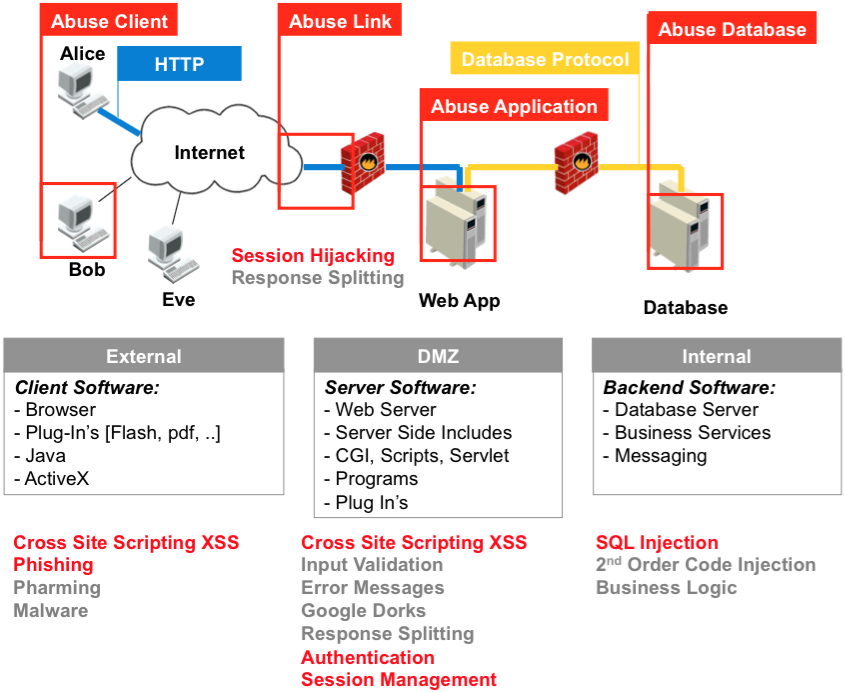
\includegraphics[width=\columnwidth]{img/webapp-threatvectors.png}
  }

  \sectionbox {
  \subsection{HTTP and Session Management}
    HTTP is stateless $\ra$ state needs to be implemented with session ID

    \textbf{SessionID}: generated on server, stored on client, transmitted with every request

    After login $\ra$ Identification by SessionID (Target for attacker)

  \subsubsection{Generation}
  \begin{itemize}
    \item Strong $\ra$ not predictive + impossible to guess next value
    \item Random $\ra$ not based on predictable values (no MD5 or SHA-1)
  \end{itemize}

  \subsubsection{Transport}
    \begin{itemize}
      \item GET: easy (in URL), compatible(+) , logged(-), HTTP referer(-)
      \item POST: compatible(+)(works with cookies disabled), not obvious(+), more complex development(-), slightly harder to manipulate(-)
      \item Cookie: more options(+), not recorded(+), https restriction(+), store on client(-), may be disabled by users(-)
    \end{itemize}

  \subsubsection{Revocation}
  \begin{itemize}
    \item Session Validity: client and server side revocation + time limited
    \item Session Timeout: important with shared computers, expiry time should be minimum
  \end{itemize}

  \subsubsection{Destruction}
  ??? %TODO See if we need to add something in Destruction
  }

  \sectionbox {
  \subsection{Attacks}
    \begin{itemize}
      \item Network sniffing $\ra$ use HTTPS to prevent it
      \item Don't mix HTTP and HTTPS SessionID
      \item Random SessionID is important
      \item Brute Force $\ra$ Not predictable Username and Password
    \end{itemize}
  }

\section*{SQL Injection (SQLi)}
  \sectionbox{
  \subsection{Code Injection}
    Attack which insert code that is afterwards interpreted by a process.

    \textbf{Process:}
    \begin{enumerate}
      \item Data enters app from untrusted source
      \item Data is part of a string executed as a command by app
      \item App gives attacker privilege or info that he would otherwise not have
    \end{enumerate}
  }

  \sectionbox{
  \subsection{SQL code injection}
    SQLi = insertion of SQL query via input data from client to app.

    \textbf{What can you do with it ?}
    \begin{itemize}
      \item Read / Modify data in the database
      \item Execute admin operations on the DB
      \item issue commands on the OS
    \end{itemize}

    \subsubsection{Tautology}
      Inject code in conditional statement(s) $\Ra$ always evaluate to true\\
      \texttt{SELECT uid FROM users WHERE login='\textcolor{red}{' OR ''='}' AND pwd='\textcolor{red}{' OR ''='}';}

    \subsubsection{Union Query}
      Inject \texttt{UNION} query $\Ra$ get union of the 2 queries\\
      \texttt{SELECT uid FROM users WHERE login=’\textcolor{red}{’ UNION SELECT cardNo from CreditCards WHERE uid=123; --} AND pass=’’;}

    \subsubsection{Piggy-Backed Queries}
      Inject query at the end of another query ($\Leftarrow$ Misconfiguration)\\
      \texttt{SELECT * FROM users WHERE uid=’abc’ AND password=’\textcolor{red}{’; DROP TABLE users; --}';}

    \subsubsection{Stored Procedure}
      Execute stored procedures present in the database\\
      \texttt{SELECT * FROM users WHERE uid=’abc’ AND password=’\textcolor{red}{’; SHUTDOWN; --}';}

    \subsubsection{Inference}
      If DB doesn't return error msg $\Ra$ change behaviour of DB to guess (Blind Injection or Time Injection (e.g. example)\\
      \url{http://www.example.com/product.php?product_id=}\texttt{\textcolor{red}{100 AND IF(version() like ‘5\%’, sleep(15), ‘false’));--}}\\
      $\ra$ check MySQL version 5.x or not $\Ra$ if yes server delays answer 15s


    \subsubsection{Alternate Encodings}
    Fool scanning and detecting techniques with alternate encoding.\\
    \texttt{SELECT * FROM users WHERE uid=’abc’ AND password=’\textcolor{red}{’; exec(char(Ox73687574646f776e)); --}'}

    \begin{itemize}
      \item \texttt{;} $\ra$ terminates a command
      \item \texttt{--} $\ra$ considers everything afterwards as a comment.
      \item Error messages can provide hints on which DB is used.
      \item \textbf{IDS Detection} can be avoided by varying the command (e.g. through the insertion of whitespaces)
    \end{itemize}
  }

  \sectionbox{
  \subsection{SQL Injection Defense}
    \begin{itemize}
    \item constrain and sanitize all client data on the server
    \item use stored procedures (restraint possible actions)
    \item avoid disclosing error information
    \item run DB with reduced privileges
    \end{itemize}
  }

\section*{Cross-Site Scripting (XSS)}
  \sectionbox{
    \subsection{Same-origin policy}
      A script can only access content and properties of a document loaded from the same origin ($\Leftrightarrow$ same protocol, same hostname, same port but ignoring URL path)

      \textbf{Interaction of different origins}
      \begin{itemize}
        \item Link (href)
        \item iframe: Shown inside the website but can't exit iframe
        \item POST: POSTing data to external source (php form \ldots)
        \item script included: Evaluated in context of the website ($\Ra$ Dangerous)
        \item Asynchronous Requests (AJAX): Different origin only possible if allowed by target domain (with Access-Control-Allow-Origin Header)
      \end{itemize}
  }

  \sectionbox{
  \subsection{XSS Attacks}
    XSS flaws occur whenever a web app takes user supplied datas and sends it to another web browser without first \emph{validating} or \emph{encoding} the content ($\Ra$ allows injection of malicious code).

    \textbf{Target:} The user of the web app

    \textbf{Infection path:} email, chat, uploaded files \ldots

    \textbf{Dangerous content:} advertisements, user contributed content, widgets (counters, scripts \ldots)

    \textbf{Example}: Data Leakage = script reads session cookies and sends them to an evil server ($\ra$ Solution: HTTPOnly cookies)

    \subsubsection{Countermeasures}
      \begin{itemize}
        \item Test your web app
        \item Input sanitization (check user submitted content)
        \item HTML output encoding (escaping)
      \end{itemize}
  }

  \sectionbox{
  \subsection{Request Forgery (XSRF)}
    A form from one domain posts a request to a different domain through an authenticated session (= write-only attack)

    \textbf{Countermeasures:} CSRF Token, ask for old password, check HTTP referer, show captcha
  }

  \sectionbox{
  \subsection{Script inclusion (XSSI)}
    \emph{Never include a script you do not trust!}

    \textbf{Direct sourcing}: honest server includes untrusted code from an external source

    \textbf{Call-back}: attacker’s website includes code (e.g.: scripts to send money) from an honest server which do not verify that the user really intended to execute it.

    \textbf{Countermeasures:} security tokens derived from the cookie and a server challenge, use only HTTP POST, check HTTP referer
  }

% Malware
\section{Malware}

  \sectionbox{
  \subsection{Definitions}
    \textbf{Malicious software (Malware)} is software that is intentionally included or inserted in a computer system for a harmful purpose.

    \textbf{Trojan}: seemingly offers useful functionalities but contains hidden functionality which undermine system security

    \textbf{Worm}: Software that can replicate itself from computer to computer across network connections

    \textbf{Bot}: malicious software agent running on a compromised machine executing commands by the bot master by listening to the command and control center (\textbf{botnet}= all bots listening to the same C\&C)

    \textbf{Rootkit}: activate during boot, hides from OS

    \textbf{Keylogger}: records keys pressed to steal information

    \textbf{Ransomware}: encrypt data and extort money for decryption key
  }

  \sectionbox{
  \subsection{Malware on Portable Storage}
    \begin{itemize}
      \item Uses Sneakernet(people) as physical propagation
      \item Variants: boot code virus (replaces boot sector), host program infection (embedding into executables)
    \end{itemize}
  }

  \sectionbox{
  \subsection{Problem of malware}

  \begin{itemize}
    \item Unauthorized use of system/network resources
    \item Sabotage
    \item Espionage
    \item Lowering of system security
  \end{itemize}
  }

  \sectionbox{
  \subsection{Malware detection}
    \textbf{Goal:} Detect malware and disinfect system

    \textbf{Deployment:} Endpoint, Network

    \textbf{Evaluation:} Recognition rate (high true positive), False alarm rate

    \subsubsection{Signature Based}
      \begin{itemize}
        \item Reactive (based on known malware binaries)
        \item Signature database (keeps growing, polymorphism)
        \item Metrics: update delay, coverage, resource consumption
       \end{itemize}

    \subsubsection{Behaviour Based}
      \begin{itemize}
        \item Requires behavior model (ground truth, baseline)
        \item Problematic: user alerting (when is it a problem ?)
       \end{itemize}

     \subsubsection{Evaluation Antivirus Softwares}
        \begin{itemize}
          \item Detection (reactive, proactive)
          \item Support for compression
          \item Self-protection
          \item Cleanup
          \item Enterprise deployment features
        \end{itemize}
  }

  \sectionbox{
  \subsection{Resistant Malware}
    \subsubsection{Antivirus Detection Evasion}
      \begin{itemize}
         \item Polymorphism (signature won't recognize them)
         \item Code obfuscation (Disguise actual purpose)
         \item Encryption of code and messages
         \item Code changes to prevent disassembly
         \item Sandbox detection (act normal if monitored)
         \item Bootstrapping / Multi Stage Worms
       \end{itemize}

    \subsubsection{Advanced Persistent Threat (APT)}
      Sophisticated stealth customized attack on selected high value targets
      \begin{itemize}
        \item \textbf{Advanced}: sophisticated attack techniques
        \item \textbf{Persistent}: might launch any time and hide well, hard to detect
        \item \textbf{Threat}: specific objective, skilled, well funded
      \end{itemize}

      \textbf{Examples}: Aurora(2009) open backdoor, Stuxnet(2010)
  }

  \sectionbox{
    \subsection{Worm Propagation Mechanism}
      \begin{enumerate}
        \item Select a target host address (hitlist, random scanning\ldots)
        \item Contact target host
        \item Check if target is vulnerable
        \item Exploit vulnerability
        \item Install copy of worm
        \item Start copy
        \item Goto 1
      \end{enumerate}

      \textbf{Propagation speed}: scan rate, vulnerable population, system compromise delay, worm transfer speed

      \subsubsection{SIS Model (Susceptible-Infected-Susceptible)}
        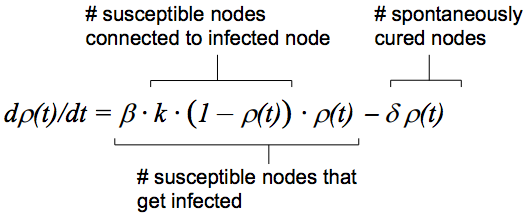
\includegraphics[scale=0.3]{img/SISmodel.png}

        \begin{itemize}
          \item Only two possible states: Susceptible or Infected
          \item $\rho(t)$ fraction of infected nodes
          \item $\beta$: infection rate
          \item $\delta$: cure rate
          \item $k$: number of outgoing edges at each node
        \end{itemize}
  }

  \sectionbox{
    \subsection{Worm Network Impact}
      Primary network impact is due to scanning activity
      \begin{itemize}
        \item ARP flooding
        \item High volume of ICMP destination unreachable msg
        \item Higher network and traffic flows
       \end{itemize}
  }

  \sectionbox{
    \subsection{Malware countermeasures}
     \begin{itemize}
        \item End system: patching, firewall, IPS, Antivirus
        \item Anti-Virus: useful but not too effective
        \item Monocultures are targeted first (e.g. Windows)
        \item Slow patching is a huge risk
        \item Application whitelisting
        \item No trusted intranet
        \item Thin Client (e.g. ChromeOS)
      \end{itemize}
  }

\section{Botnets + Malware Development}
  \sectionbox{
  \subsection{Objectives to best utilize infected machines}
    \begin{itemize}
      \item \textbf{Buildup} efficient infection and spreading
      \item \textbf{Persistence}: prevent detection and Removal
      \item \textbf{Modularity}: address changing functionality needs
      \item \textbf{Scalability}: handle large number of machines
      \item \textbf{Adaptive}: to business and technology challenges
      \item \textbf{Anonymity}: prevent identification of operator
    \end{itemize}
  }

  \sectionbox{
    \subsection{Target exploitation}
    \begin{itemize}
      \item \textbf{Persist and avoid detection}: explore, steal information, load functionality, maximize yield
      \item \textbf{Move to active attacks}: load attack functionality $\ra$ higher chance of detection
      \item \textbf{Throw away agent}: sell to idiots
    \end{itemize}
  }

  \sectionbox{
  \subsection{Bot Command Modes}
    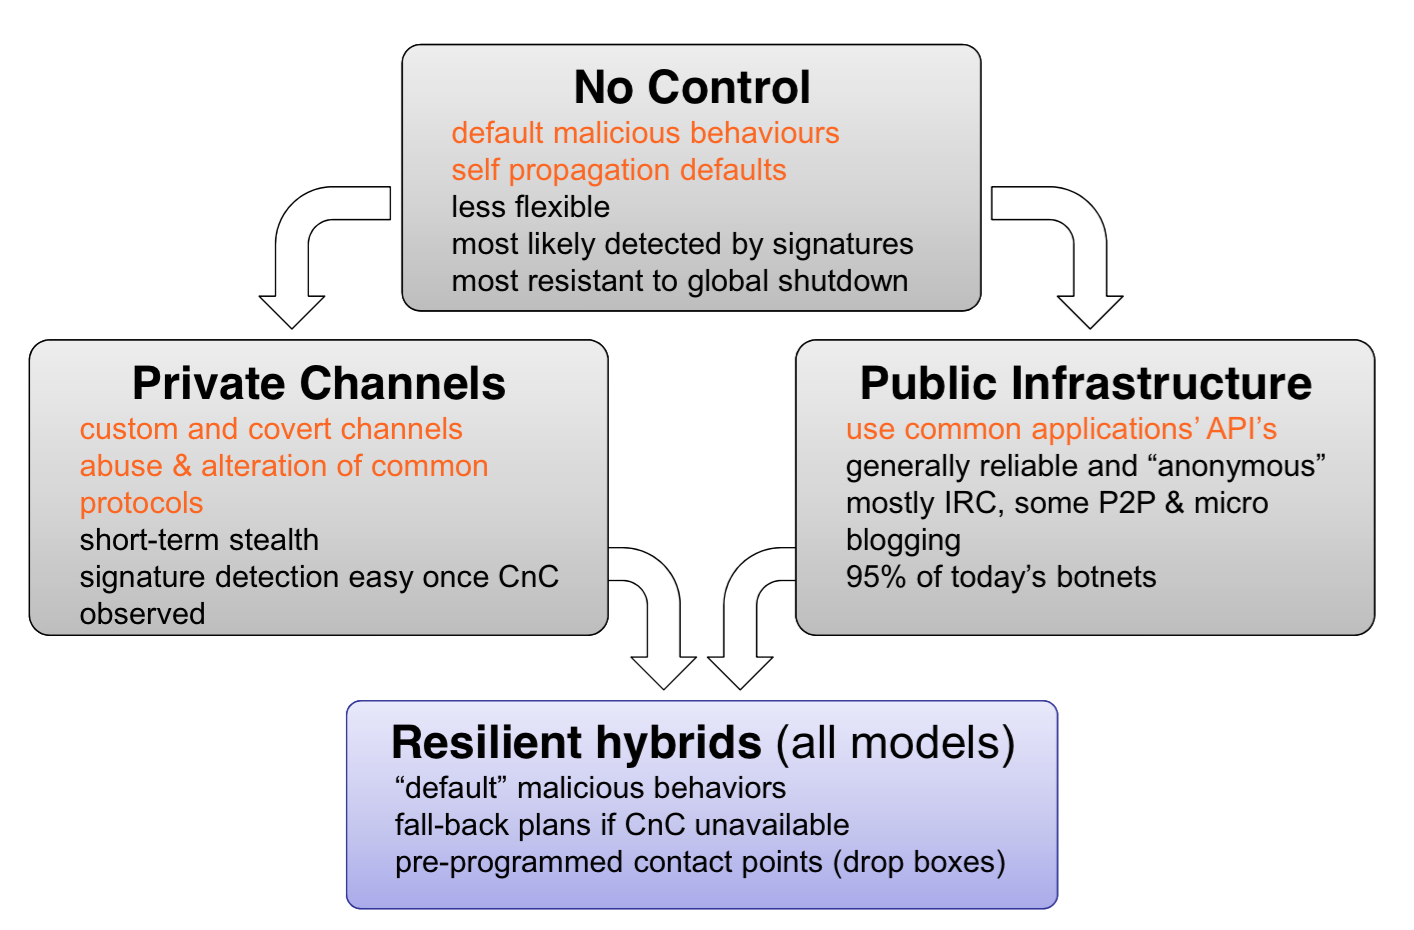
\includegraphics[width=\columnwidth]{img/bot-command-modes.png}
  }

  \sectionbox{
  \subsection{Exploitation Phases}
    \begin{enumerate}
      \item ID Theft (Keylogger, sniffer\ldots)
      \item Peer and Social Attacks (Trust misuse)
      \item Local Attacks (Local Network, USB, VPN)
      \item Attack Support (Host of Phishing Site, Proxying)
      \item External/Noisy Attacks (Scanning, Spam, DDoS)
    \end{enumerate}

    \textbf{CnC Topologies:} Star, multi-server, hierarchical, random
  }

  \sectionbox{
  \subsection{CnC Topology}
    \begin{itemize}
      \item \textbf{Star}: Single centralized CnC (+ Speed of control, - 1 point of failure)
      \item \textbf{Multi-server}: Multiple CnC communicating together (+ No single point of failure, + Geographical optimization, - Advanced planning required)
      \item \textbf{Hierarchical}: Multiple layers below CnC (+ Botnet awareness, Ease or resale, - Latency)
      \item \textbf{Random}: No centralized CnC (+ Highly resilient, - Latency,
      - Botnet enumeration)
    \end{itemize}
  }

  \sectionbox{
  \subsection{Fluxing Technologies}
  \begin{itemize}
    \item \textbf{IP-Flux}: Constant change of IP address information related to a particular fully-qualified domain name (FQDN) (cnc.net$\ra$multiple IPs)
    \item \textbf{Domain Flux}: Constant change and allocation of multiple fully-qualified domain names (FQDN) (cnc.net, cnc.ru, abc.net$\ra$ multiple IPs)
    \item \textbf{Single-Flux}: The FQDN of the CnC’s host has multiple IPs addresses assigned (DNS A record)
    \item \textbf{Double-Flux}: The name servers of the CnC’s FQDN as well as the FQDN of the CnC’s host have multiple IP addresses assigned (DNS A and NS records)
  \end{itemize}
  }

  \sectionbox{
  \subsection{Malware Development Process}
    \begin{enumerate}
      \item \textbf{Create} unique samples of malware at \underline{massive scale}
      \item \textbf{Crypter}: encrypt malware to protect against signature detection
      \item \textbf{Protector}: prevent debugging (against reverse engineering, sandboxing)
      \item \textbf{Packers}: make it smaller + use polymorphism
      \item \textbf{Binders}: hide it in another application
      \item \textbf{Quality Assurance}: Test detectability before deployment
    \end{enumerate}
  }

  \sectionbox{
  \subsection{Takedown}
    Legal and technical measures to sever the connection between the CnC structure and the bot agents
  }

  \sectionbox{
  \subsection{Defense}
    \begin{itemize}
      \item Firewalls
      \item Antivirus (up-to-date) but know its limits
      \item Patch your system
      \item brain.exe
    \end{itemize}
  }

% Security Ecosystem and Detection Failures
\section{Security Ecosystem and Detection Failures}

  \emphbox{A vulnerability is a weakness in software (or hardware) that enables an attacker to compromise the software or the data that it processes}
  \sectionbox{
  \subsection{Security Information Provider}
    SIP: Organizations that efficiently monitor the primary sources of security information, validate the content found, and publish their findings as security advisories in a consistent format (NVD, CVE)
  }
  \sectionbox{
    \subsection{Disclosure Options}
    \begin{itemize}
      \item Exploit
      \item Sell on Black Market
      \item Full Disclosure
      \item Coordinated/Responsible Disclosure
      \item Sell on White Market
    \end{itemize}
  }

% E-Mail Spam
\section{E-Mail Spam}
  \sectionbox{
  \subsection{Generalities about Spam}
    \subsubsection{Types of Spam}
      \textbf{UCE}: Unsolicited Commercial Email

      \textbf{UBE}: Unsolicited Bulk Email (not necessarily commercial)

    \subsubsection{Where to get emails addresses}
      \begin{itemize}
        \item Directory Harvest Attack (DHA) against mail server
        \item Email address crawlers
        \item Malware
        \item Harvesting email addresses from databases
      \end{itemize}

    \subsubsection{Spam Sending Tactics}
      \begin{itemize}
        \item Send from borrowed email accounts
        \item Send from short-term officially registered domain
        \item Use fake sender domains
        \item Sending spam from botnet machines
        \item Open mail relays (anyone can do it)
        \item Open proxies
      \end{itemize}
  }

  \sectionbox{
  \subsection{Anti-Spam Techniques}
    \begin{itemize}
      \item \textbf{Filter at SMTP time}: lack info. to decide
      \item \textbf{DNS Blacklists}:
        \begin{itemize}
          \item Greylisting: defer 1st email but accept follow-up email (issues with delays and multiple SMTP hosts of larger hosters)
          \item Blacklisting(DNSBL): can be done either with IP or domain name
        \end{itemize}
      \item \textbf{Filtering SMTP traffic at FW}: block outgoing SMTP msg not from SMTP server (prevent email-based worms)
      \item \textbf{Heuristical Content Filtering}: look at weird font, strange URL \ldots)
      \item \textbf{Statistical Content Filtering}:\\
      $P(spam|words) = \frac{P(words|spam)P(spam)}{P(words)}$
      \item \textbf{Traffic Based Filtering}: Compare flux of emails to recognize bulk mail (DCC = Distributed Checksum Clearinghouse)
      \item \textbf{Image Spam Filtering}: OCR on images before filtering
      \item \textbf{Text Filtering Caveats}: Normalize content before filtering text
    \end{itemize}
  }

  \sectionbox{
  \subsection{Email Authentication}
    \begin{itemize}
      \item \textbf{S/MIME}(Secure/MIME): sign and encrypt only msg content (not header)
      \item \textbf{PGP}(Pretty Good Privacy): auth + encry with Web of Trust
      \item \textbf{DKIM}(DomainKeys Identified Mail): Sign mails between servers
      \item \textbf{SPF}(Sender Policy Framework): List of IPs allowed to send emails
      \item \textbf{SenderID}: Match PRA domain against source IP via DNS (PRA is often From: header)
    \end{itemize}

    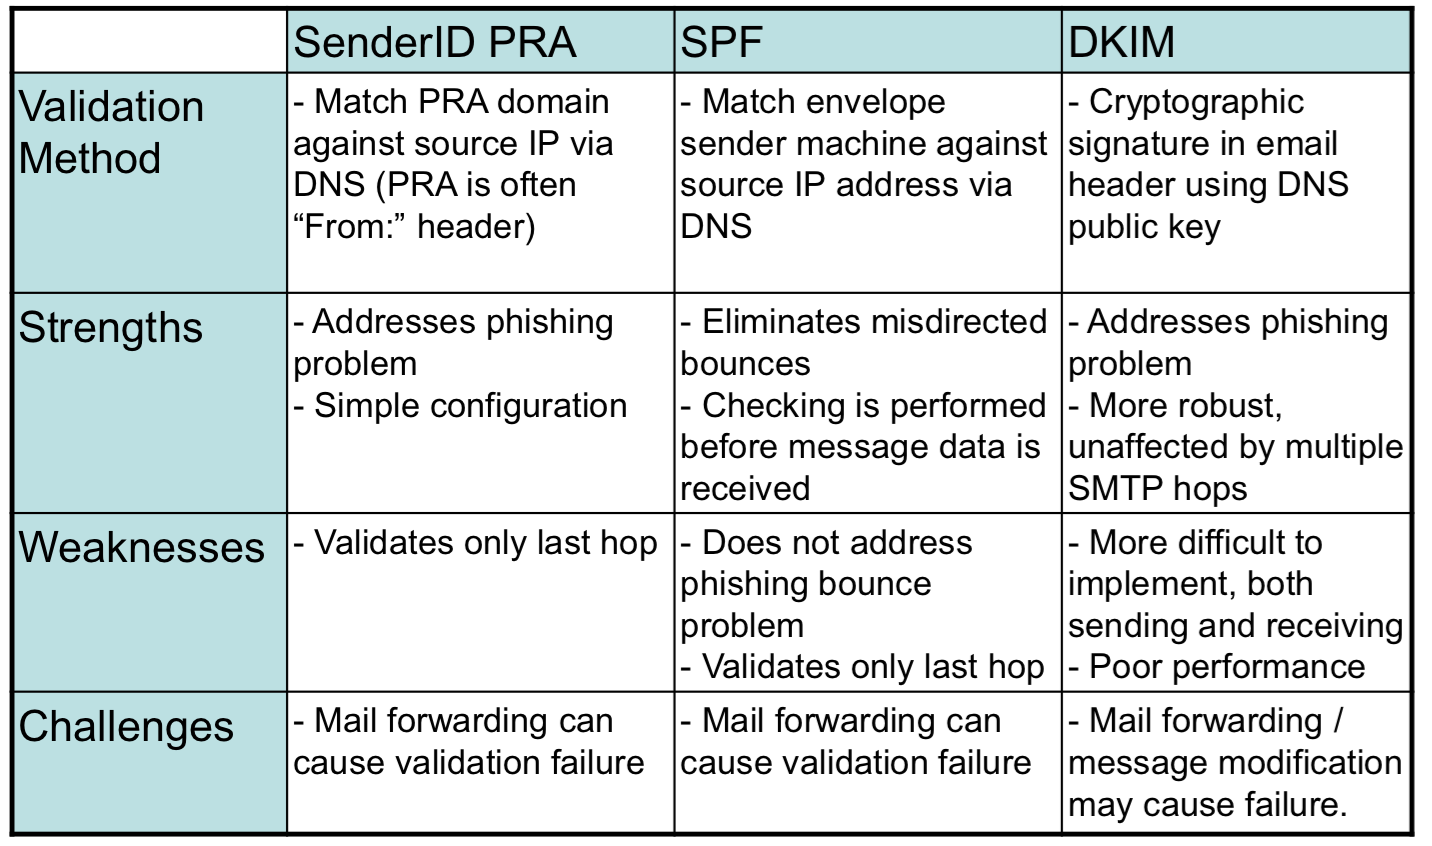
\includegraphics[width=\columnwidth]{img/emailauth.png}
  }

\section{Guest Lectures}
  \sectionbox {
  \subsection{DMZ}
    Compromised hosts in DMZ are no danger for internal network e.g.:(external - webserver(dmz) - database(internal))
  }
  \sectionbox {
  \subsection{Certificate Transparency  main goals}
    \begin{itemize}
      \item Make it impossible (or at least very difficult) for a CA to issue a SSL certificate for a domain without the certificate being visible to the owner of that domain.
      \item Provide an open auditing and monitoring system that lets any domain owner or CA determine whether certificates have been mistakenly or maliciously issued.
      \item Protect users from being duped by certificates that were mistakenly or maliciously issued.
    \end{itemize}
}

\end{document}
